\documentclass[doc,floatsintext]{apa6}
\usepackage{lmodern}
\usepackage{amssymb,amsmath}
\usepackage{ifxetex,ifluatex}
\usepackage{fixltx2e} % provides \textsubscript
\ifnum 0\ifxetex 1\fi\ifluatex 1\fi=0 % if pdftex
  \usepackage[T1]{fontenc}
  \usepackage[utf8]{inputenc}
\else % if luatex or xelatex
  \ifxetex
    \usepackage{mathspec}
  \else
    \usepackage{fontspec}
  \fi
  \defaultfontfeatures{Ligatures=TeX,Scale=MatchLowercase}
\fi
% use upquote if available, for straight quotes in verbatim environments
\IfFileExists{upquote.sty}{\usepackage{upquote}}{}
% use microtype if available
\IfFileExists{microtype.sty}{%
\usepackage{microtype}
\UseMicrotypeSet[protrusion]{basicmath} % disable protrusion for tt fonts
}{}
\usepackage{hyperref}
\hypersetup{unicode=true,
            pdftitle={Help, My Collaborator Uses R! An Introduction to Reproducible Statistical Analyses in R},
            pdfauthor={Wouter de Nooy~\& Second (Third, \ldots{}) Author},
            pdfkeywords={R; statistical analyses; reproducible research; R Markdown},
            pdfborder={0 0 0},
            breaklinks=true}
\urlstyle{same}  % don't use monospace font for urls
\usepackage{color}
\usepackage{fancyvrb}
\newcommand{\VerbBar}{|}
\newcommand{\VERB}{\Verb[commandchars=\\\{\}]}
\DefineVerbatimEnvironment{Highlighting}{Verbatim}{commandchars=\\\{\}}
% Add ',fontsize=\small' for more characters per line
\usepackage{framed}
\definecolor{shadecolor}{RGB}{248,248,248}
\newenvironment{Shaded}{\begin{snugshade}}{\end{snugshade}}
\newcommand{\KeywordTok}[1]{\textcolor[rgb]{0.13,0.29,0.53}{\textbf{#1}}}
\newcommand{\DataTypeTok}[1]{\textcolor[rgb]{0.13,0.29,0.53}{#1}}
\newcommand{\DecValTok}[1]{\textcolor[rgb]{0.00,0.00,0.81}{#1}}
\newcommand{\BaseNTok}[1]{\textcolor[rgb]{0.00,0.00,0.81}{#1}}
\newcommand{\FloatTok}[1]{\textcolor[rgb]{0.00,0.00,0.81}{#1}}
\newcommand{\ConstantTok}[1]{\textcolor[rgb]{0.00,0.00,0.00}{#1}}
\newcommand{\CharTok}[1]{\textcolor[rgb]{0.31,0.60,0.02}{#1}}
\newcommand{\SpecialCharTok}[1]{\textcolor[rgb]{0.00,0.00,0.00}{#1}}
\newcommand{\StringTok}[1]{\textcolor[rgb]{0.31,0.60,0.02}{#1}}
\newcommand{\VerbatimStringTok}[1]{\textcolor[rgb]{0.31,0.60,0.02}{#1}}
\newcommand{\SpecialStringTok}[1]{\textcolor[rgb]{0.31,0.60,0.02}{#1}}
\newcommand{\ImportTok}[1]{#1}
\newcommand{\CommentTok}[1]{\textcolor[rgb]{0.56,0.35,0.01}{\textit{#1}}}
\newcommand{\DocumentationTok}[1]{\textcolor[rgb]{0.56,0.35,0.01}{\textbf{\textit{#1}}}}
\newcommand{\AnnotationTok}[1]{\textcolor[rgb]{0.56,0.35,0.01}{\textbf{\textit{#1}}}}
\newcommand{\CommentVarTok}[1]{\textcolor[rgb]{0.56,0.35,0.01}{\textbf{\textit{#1}}}}
\newcommand{\OtherTok}[1]{\textcolor[rgb]{0.56,0.35,0.01}{#1}}
\newcommand{\FunctionTok}[1]{\textcolor[rgb]{0.00,0.00,0.00}{#1}}
\newcommand{\VariableTok}[1]{\textcolor[rgb]{0.00,0.00,0.00}{#1}}
\newcommand{\ControlFlowTok}[1]{\textcolor[rgb]{0.13,0.29,0.53}{\textbf{#1}}}
\newcommand{\OperatorTok}[1]{\textcolor[rgb]{0.81,0.36,0.00}{\textbf{#1}}}
\newcommand{\BuiltInTok}[1]{#1}
\newcommand{\ExtensionTok}[1]{#1}
\newcommand{\PreprocessorTok}[1]{\textcolor[rgb]{0.56,0.35,0.01}{\textit{#1}}}
\newcommand{\AttributeTok}[1]{\textcolor[rgb]{0.77,0.63,0.00}{#1}}
\newcommand{\RegionMarkerTok}[1]{#1}
\newcommand{\InformationTok}[1]{\textcolor[rgb]{0.56,0.35,0.01}{\textbf{\textit{#1}}}}
\newcommand{\WarningTok}[1]{\textcolor[rgb]{0.56,0.35,0.01}{\textbf{\textit{#1}}}}
\newcommand{\AlertTok}[1]{\textcolor[rgb]{0.94,0.16,0.16}{#1}}
\newcommand{\ErrorTok}[1]{\textcolor[rgb]{0.64,0.00,0.00}{\textbf{#1}}}
\newcommand{\NormalTok}[1]{#1}
\usepackage{graphicx,grffile}
\makeatletter
\def\maxwidth{\ifdim\Gin@nat@width>\linewidth\linewidth\else\Gin@nat@width\fi}
\def\maxheight{\ifdim\Gin@nat@height>\textheight\textheight\else\Gin@nat@height\fi}
\makeatother
% Scale images if necessary, so that they will not overflow the page
% margins by default, and it is still possible to overwrite the defaults
% using explicit options in \includegraphics[width, height, ...]{}
\setkeys{Gin}{width=\maxwidth,height=\maxheight,keepaspectratio}
\IfFileExists{parskip.sty}{%
\usepackage{parskip}
}{% else
\setlength{\parindent}{0pt}
\setlength{\parskip}{6pt plus 2pt minus 1pt}
}
\setlength{\emergencystretch}{3em}  % prevent overfull lines
\providecommand{\tightlist}{%
  \setlength{\itemsep}{0pt}\setlength{\parskip}{0pt}}
\setcounter{secnumdepth}{5}
% Redefines (sub)paragraphs to behave more like sections
\ifx\paragraph\undefined\else
\let\oldparagraph\paragraph
\renewcommand{\paragraph}[1]{\oldparagraph{#1}\mbox{}}
\fi
\ifx\subparagraph\undefined\else
\let\oldsubparagraph\subparagraph
\renewcommand{\subparagraph}[1]{\oldsubparagraph{#1}\mbox{}}
\fi

%%% Use protect on footnotes to avoid problems with footnotes in titles
\let\rmarkdownfootnote\footnote%
\def\footnote{\protect\rmarkdownfootnote}


  \title{Help, My Collaborator Uses R! An Introduction to Reproducible
Statistical Analyses in R}
    \author{Wouter de Nooy\textsuperscript{1}~\& Second (Third, \ldots{})
Author\textsuperscript{1,2}}
    \date{}
  
\shorttitle{Help, My Collaborator Uses R!}
\affiliation{
\vspace{0.5cm}
\textsuperscript{1} Amsterdam School of Communication Research ASCoR\\\textsuperscript{2} University of Amsterdam}
\keywords{R; statistical analyses; reproducible research; R Markdown\newline\indent Word count: (to be added manually)}
\usepackage{csquotes}
\usepackage{upgreek}
\captionsetup{font=singlespacing,justification=justified}

\usepackage{longtable}
\usepackage{lscape}
\usepackage{multirow}
\usepackage{tabularx}
\usepackage[flushleft]{threeparttable}
\usepackage{threeparttablex}

\newenvironment{lltable}{\begin{landscape}\begin{center}\begin{ThreePartTable}}{\end{ThreePartTable}\end{center}\end{landscape}}

\makeatletter
\newcommand\LastLTentrywidth{1em}
\newlength\longtablewidth
\setlength{\longtablewidth}{1in}
\newcommand{\getlongtablewidth}{\begingroup \ifcsname LT@\roman{LT@tables}\endcsname \global\longtablewidth=0pt \renewcommand{\LT@entry}[2]{\global\advance\longtablewidth by ##2\relax\gdef\LastLTentrywidth{##2}}\@nameuse{LT@\roman{LT@tables}} \fi \endgroup}


\geometry{a4paper, top=30mm, bottom = 25mm, asymmetric = FALSE}
\usepackage{float}
\usepackage{wrapfig}

\authornote{Add complete departmental affiliations for each
author here. Each new line herein must be indented, like this line.
Enter author note here.

Correspondence concerning this article should be addressed to Wouter de
Nooy, Nieuwe Achtergracht 166, 1018 WV Amsterdam. E-mail:
\href{mailto:w.denooy@uva.nl}{\nolinkurl{w.denooy@uva.nl}}}

\abstract{
This is a concise introduction to using R for reproducible statistical
analyses. It is meant to function as a guide and reference work for
researchers who start using R and R Markdown or who have not used R or R
Markdown for some time.

This document itself uses R for analyses and it is written in R
Markdown. As such, it exemplifies the topics that it discusses. The R
Markdown document can be downloaded from
\url{https://wdenooy.github.io/Switch2R/HelpMyCollaboratorUsesR.Rmd}.
The PDF version is available at
\url{https://wdenooy.github.io/Switch2R/HelpMyCollaboratorUsesR.pdf}.


}

\begin{document}
\maketitle

\section{Why Use R?}\label{why-use-r}

Because you want to be one of the nerds. Instead of publicly
acknowledging this deep-felt need, you resort to arguments such as:

\begin{itemize}
\tightlist
\item
  I want to be up-to-date. The latest developments in data handling and
  analysis are implemented (first) in R.
\item
  I want to do all my work in one environment. From data scraping via
  all kinds of analyses to publishing papers and books, all can be done
  in R.
\item
  I want my analyses to be reproducible. All steps from data cleaning to
  final results can be specified and documented in one document in R.
\item
  I want to be in full control of my analyses, tables, and figures. I do
  not want to depend on defaults set by the software creator.
\item
  I want to use free, open source software, so everybody can check and
  improve my work.
\end{itemize}

\section{Start Working with R}\label{start-working-with-r}

In contrast to SPSS, R (R Core Team,
\protect\hyperlink{ref-R-base}{2019}) is not a single software package
(well, neither is SPSS but we usually install all licensed SPSS parts)
and it does not have an attractive user interface. Working with R, you
may have to install additional packages (also called \emph{libraries})
for doing the things that you want to do. A more user-friendly interface
to R is provided by RStudio, which is free like R. Let us install both R
and RStudio, learn how to install additional packages, and how to
operate R from within RStudio.

\subsection{Install or update R}\label{install-or-update-r}

On your \emph{private computer} or UvA \emph{self-support laptop},
download and install R directly from \url{https://cloud.r-project.org/}.

\begin{itemize}
\tightlist
\item
  Download the R version for your operating system: Linux, (Mac) OSX, or
  Windows.
\item
  Select the \texttt{base} package (or click
  \texttt{install\ R\ for\ the\ first\ time}).
\item
  Download and install it.
\end{itemize}

For a \emph{UvA-supported laptop}:

\begin{itemize}
\tightlist
\item
  Install R from the Software Center. Be sure to select the staff
  version (\emph{R-Project MDW}), which allows installing packages
  (Section \ref{packages}) locally on your computer.
\item
  Install RStudio from the Software Center.
\end{itemize}

Use the same procedure to update to a newer version of R.

If you want to know more about R and the organization behind R (CRAN),
visit \url{https://www.r-project.org/}.

\subsection{Install RStudio}\label{install-rstudio}

Install RStudio (Desktop, Open Source License) from
\url{http://www.rstudio.com/download}:

\begin{itemize}
\tightlist
\item
  Select your operating system.
\item
  Download and install.
\end{itemize}

Allow RStudio to install additional packages when it asks for permission
to do so.

\subsection{Create an RStudio Project}\label{create-an-rstudio-project}

When you start working on a new project, create a new RStudio project. A
project tells RStudio where to store and find files that you create.

Create a new project:

\begin{itemize}
\tightlist
\item
  Use the menu \emph{File\textgreater{}New Project\ldots{}} or the
  \emph{Create a project} button.
\item
  Select \emph{New Directory} to start a project in a brand new working
  directory or select \emph{Existing Directory} to create a new project
  in an existing directory.
\end{itemize}

The directory name is the name of the project. It is called
\emph{Modernisering} in Figure \ref{fig:RStudio}.

When you start RStudio, R starts automatically. The project that was
open when you last closed RStudio will be reopened. If you want to open
another project, use \emph{Open Project\ldots{}} in the \emph{File} menu
or use the drop-down list of projects in the top-right of the RStudio
interface.

Figure \ref{fig:RStudio} shows the main panels of the RStudio interface
with a project opened. It features a syntax file demonstrating some R
commands that are discussed in Section \ref{rcommands}.

\begin{figure}[H]
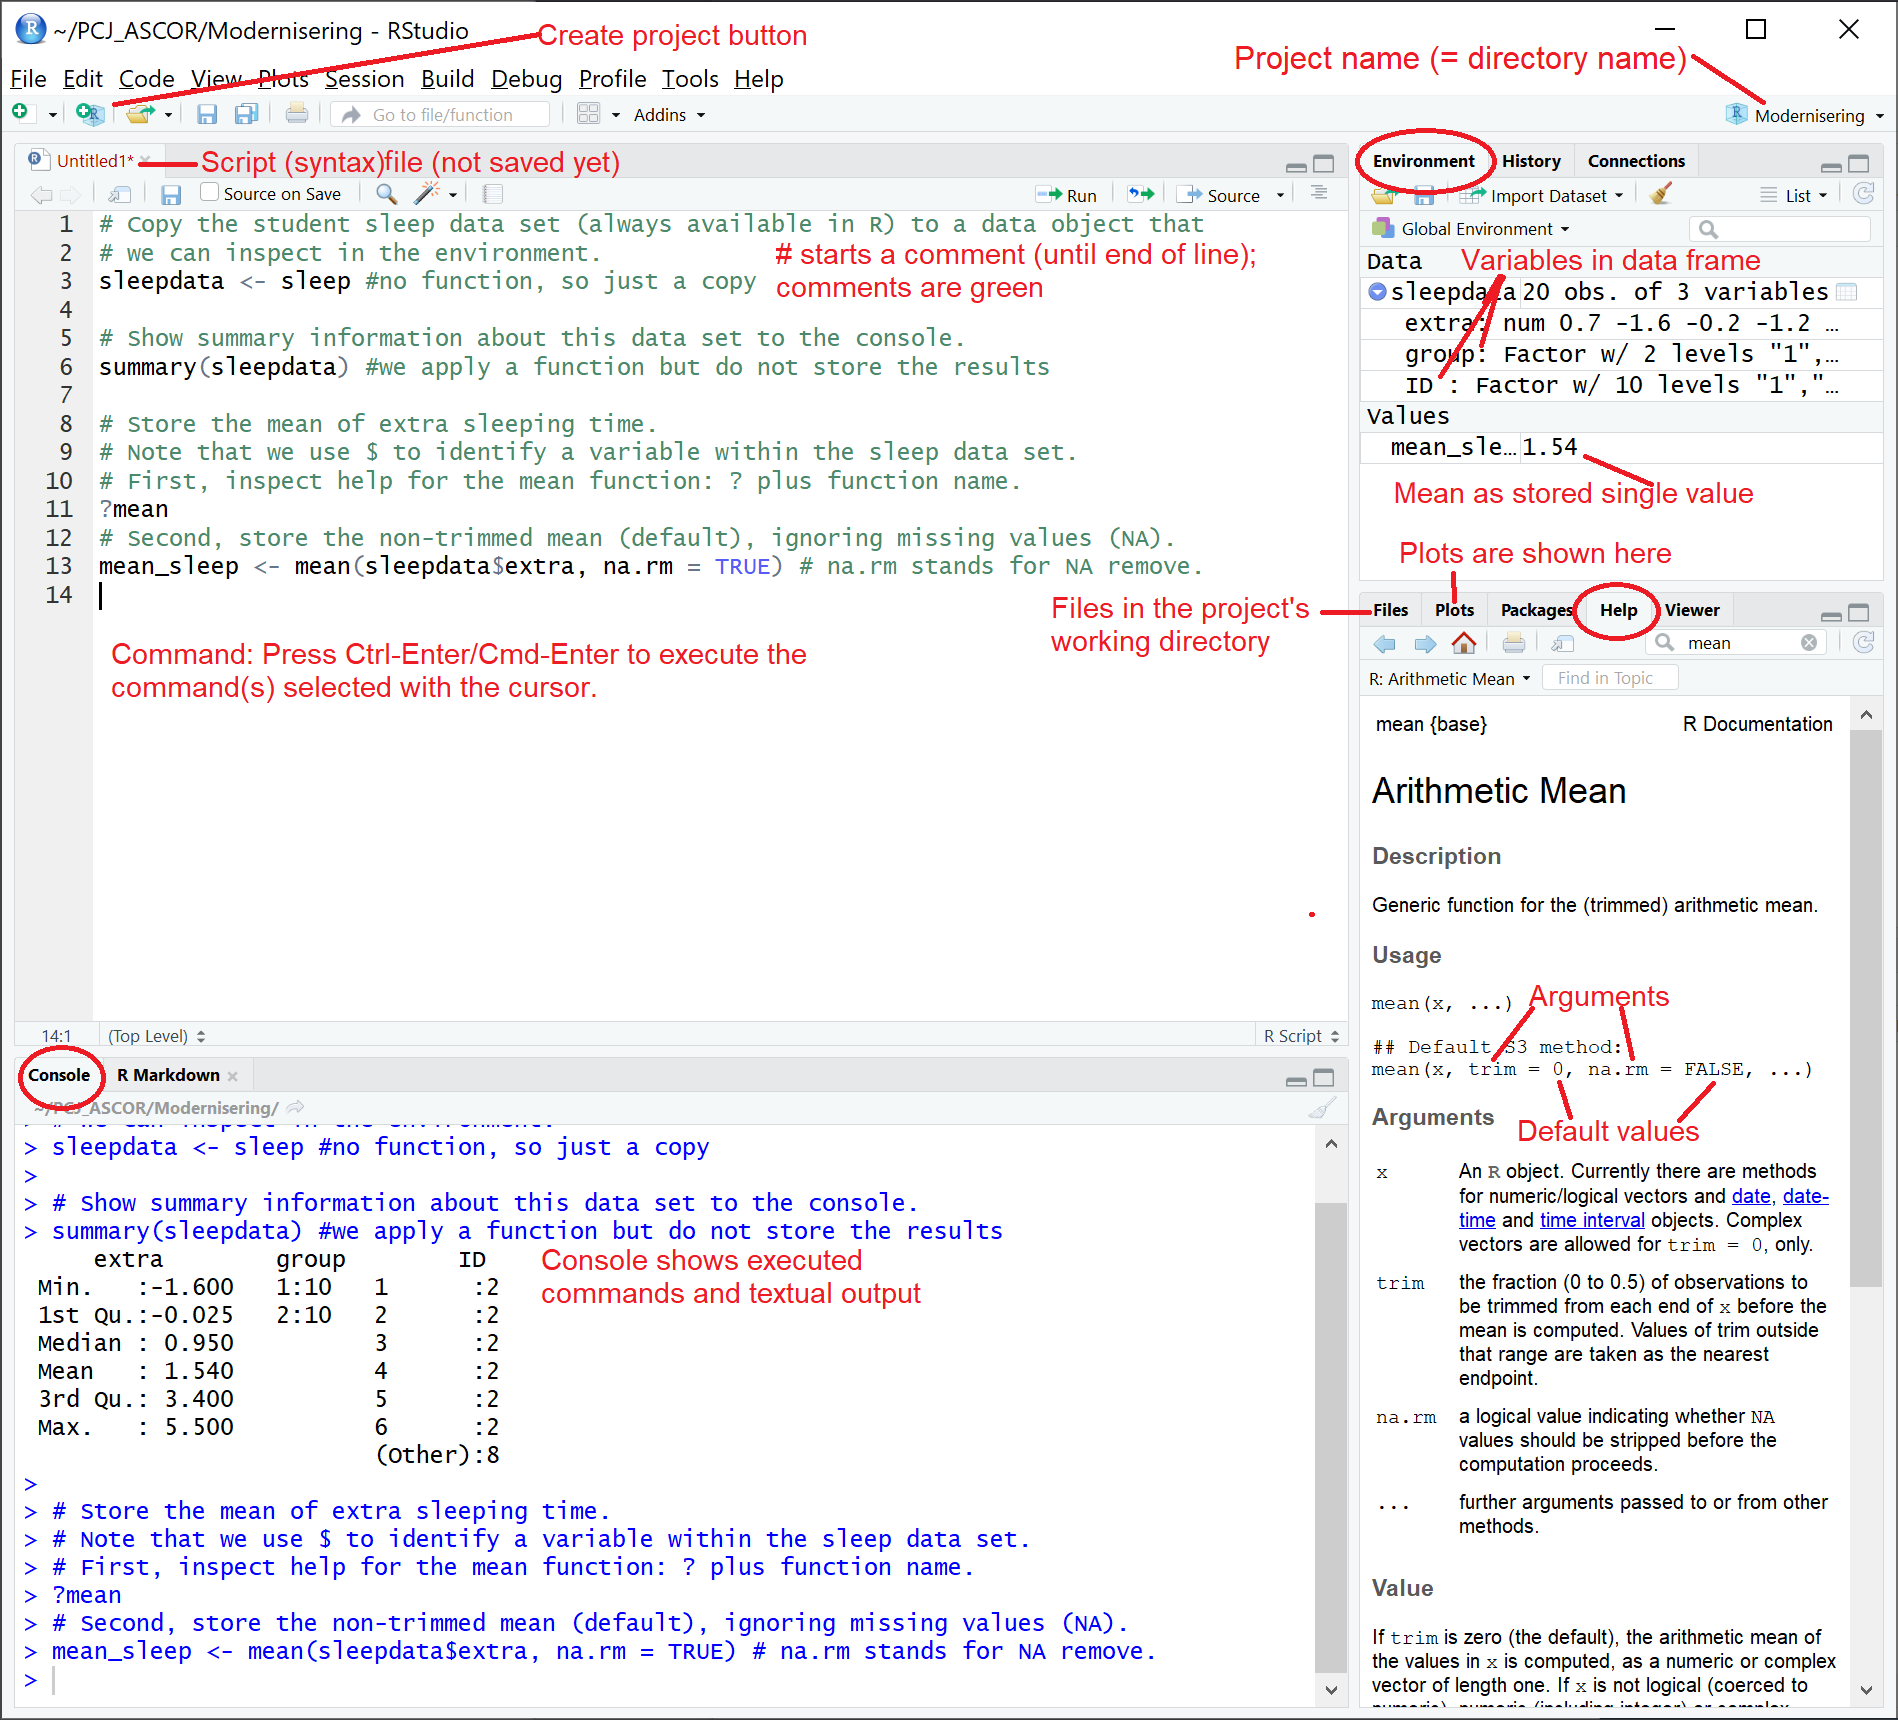
\includegraphics[width=6.33in]{RStudio} \caption{Main panels of the RStudio user interface.}\label{fig:RStudio}
\end{figure}

\subsection{Running R Commands within RStudio}\label{rcommands}

RStudio (and R) does not have a menu offering all possible data
manipulations and analyses. Instead, you have to type commands.

\subsubsection{Commands are functions}\label{commands-are-functions}

The general R layout of a command:
\texttt{y\ \textless{}-\ f(x,\ arg\ =\ z)}

This command means: Do something (function \texttt{f(arg\ =\ z)}) to
data object \texttt{x} and store the result in data object \texttt{y}.

If the left-hand data object (\texttt{y}):

\begin{itemize}
\tightlist
\item
  does not exist: a new data object is created in the project
  environment.
\item
  exists: data object is overwritten in the project environment.\\
\item
  is not named: output is sent to the screen (console or plot area).
\end{itemize}

If no function is specified, the data object (\texttt{x}) will be simply
copied to another data object or to the screen, depending on \texttt{y}.

A data object can be a data set, a list of analysis results, a function,
or (code to create) a plot. An important difference between R and SPSS
is that R stores analysis results in such a way that you can use them in
a next step of the analysis. You can extract the results that you are
interested in and use them in calculations, tables, or plots (see
Section \ref{firstanalysis}).

\subsubsection{Options are arguments to
functions}\label{options-are-arguments-to-functions}

A function can take more input from the user than just a data object
(\texttt{x}). Additional input are arguments that have a name
(\texttt{arg}, for example). The arguments for a function and their
default values are listed in the help for the function (the vignette).
The user may specify the value of arguments or rely on the default
settings.

\begin{quote}
Separate arguments and the data object by commas!
\end{quote}

Sometimes, you can supply more than one value for an argument. For
example, the \texttt{quantile()} function can calculate several
quantiles in one go. If you have to specify more than on value,
enumerate them within the \texttt{c()} function, which creates a vector
or list.

Below are some examples of commands and the textual output that the
\texttt{summary} function sends to the console, which also feature in
Figure \ref{fig:RStudio}. Note that R is case-sensitive: uppercase
letters are considered different letters than lowercase letters.

\begin{Shaded}
\begin{Highlighting}[]
\CommentTok{# Note that this code chunk is not executed (eval = FALSE). Instead, it is shown}
\CommentTok{# to the reader (echo=TRUE).}

\CommentTok{# Copy the student sleep data set (always available in R) to a data object that}
\CommentTok{# we can inspect in the environment.}
\NormalTok{sleepdata <-}\StringTok{ }\NormalTok{sleep }\CommentTok{#no function, so just a copy}

\CommentTok{# Show summary information about this data set to the console.}
\KeywordTok{summary}\NormalTok{(sleepdata) }\CommentTok{#we apply a function but do not store the results}

\CommentTok{# Store the mean of extra sleeping time.}
\CommentTok{# Note that we use $ to identify a variable within the sleep data set.}
\CommentTok{# First, inspect help for the mean function: ? plus function name.}
\NormalTok{?mean}
\CommentTok{# Second, store the non-trimmed mean (default), ignoring missing values (NA).}
\NormalTok{mean_sleep <-}\StringTok{ }\KeywordTok{mean}\NormalTok{(sleepdata}\OperatorTok{$}\NormalTok{extra, }\DataTypeTok{na.rm =} \OtherTok{TRUE}\NormalTok{) }\CommentTok{# na.rm stands for NA remove.}

\CommentTok{# Calculate the quartiles of extra sleeping time.}
\NormalTok{quartiles <-}\StringTok{ }\KeywordTok{quantile}\NormalTok{(sleepdata}\OperatorTok{$}\NormalTok{extra, }\DataTypeTok{probs =} \KeywordTok{c}\NormalTok{(}\FloatTok{0.25}\NormalTok{, }\FloatTok{0.5}\NormalTok{, }\FloatTok{0.75}\NormalTok{))}
\end{Highlighting}
\end{Shaded}

\subsubsection{Data frames are lists of
variables}\label{data-frames-are-lists-of-variables}

The \texttt{mean()} and \texttt{quartiles()} functions require a
variable: extra sleeping time (\texttt{extra}) in the example above.
Usually, variables are stored in a data frame. A data frame is (more or
less) a list of variables.

\begin{quote}
In R, you can retrieve an item from a list with the \texttt{\$}
character.
\end{quote}

We get the extra sleeping time variable (\texttt{extra}) from the
\texttt{sleepdata} data frame by first specifying the name of the data
frame, adding a dollar sign, and finally the name of the variable (list
item): \texttt{sleepdata\$extra}. If you are typing a command at the R
prompt in RStudio, a popup menu will list the items that are available
once you add the dollar sign to the name of a data frame.

Results from statistical analyses (Section \ref{firstanalysis} and on)
are also stored as lists. We can use the dollar sign to extract the
parts of the results that we are interested in.

\subsubsection{A script is a syntax file}\label{scriptfile}

Commands can be typed after the prompt (\texttt{\textgreater{}}) in the
console. Press \emph{Enter} to execute the command.

It is more efficient, however, to create a syntax file (called a script
in R) and type the commands and comments in this file. The script file
can be saved and reopened in the next R session. Select one or more
commands in the syntax file and press Ctrl-Enter or Cmd-Enter to execute
them.

Create a new script file:

\begin{itemize}
\tightlist
\item
  Use the File menu.
\item
  Select \emph{New File}.
\item
  Select \emph{R Script}.
\end{itemize}

Save script files in the default directory (this is the working
directory) and use the default file extension (\emph{.R}).

Reopen a saved script file:

\begin{itemize}
\tightlist
\item
  If the project is not open yet, open it (\emph{File \textgreater{}
  Open Project\ldots{}}).
\item
  Open the script file by clicking it in the \emph{Files} tab
  (bottom-right panel of RStudio).
\end{itemize}

Section \ref{integratingtextcode} discusses a third option for running
commands, which integrates code and text.

\subsection{Recommended RStudio settings}\label{rsettings}

\begin{wrapfigure}{r}{0.5\textwidth}
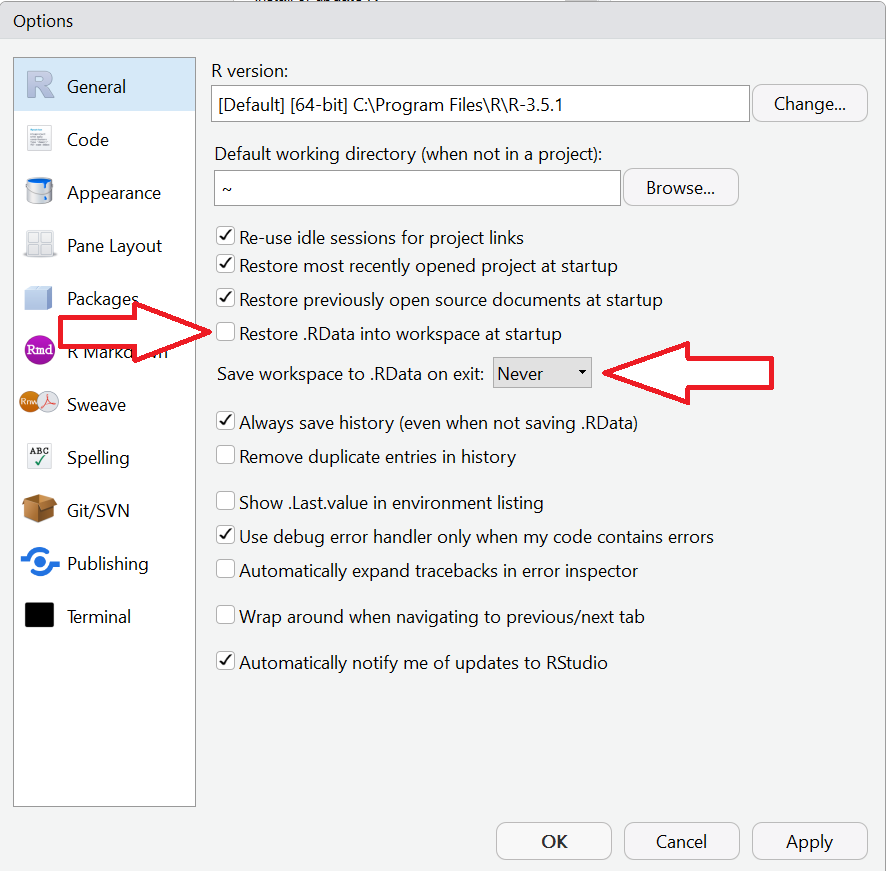
\includegraphics[width=2.96in]{Settings} \caption{Workspace settings in the Tools menu under Global Options.}\label{fig:RStudiosettings}
\end{wrapfigure}

A data object created by an R command is saved in memory, which is
called the project's environment. Data objects in the environment are
directly accessible to R.

When you exit RStudio (and R), the data objects in the environment are
deleted: memry is cleared. It is possible to save all data objects in
memory as a file on disk, which is called a \emph{work space}, with the
default file extension \emph{.RData}.

Actually, RStudio saves the work space by default when you exit RStudio.
This may sound great but it is strongly recommended NOT to save the work
space. Your R code in the syntax file should create all data objects
that you need. Your workspace, however, may contain additional objects
that you created with the console or with syntax commands that have been
removed. If you rerun the syntax when you reopen an RStudio project, you
can check that all necessary data objects are created. If not, you will
receive an error message.

For this reason, it is a good idea to turn off saving work spaces when
exiting RStudio and reloading them when reopening a project in RStudio.
To this end, adjust the settings in the \emph{Tools} menu under
\emph{Global Options} as indicated in Figure \ref{fig:RStudiosettings}.

\subsection{Install and Load Packages}\label{packages}

\begin{wrapfigure}{r}{0.3\textwidth}
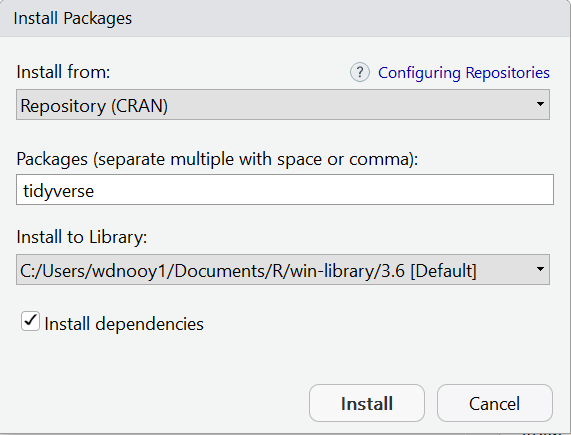
\includegraphics[width=1.9in]{installpackage} \caption{The RStudio dialog for installing packages.}\label{fig:installscreen}
\end{wrapfigure}

The base installation of R includes several important packages, such as
the \texttt{base} package and the \texttt{stats} package, which contains
many statistical analyses. These packages are loaded when you start R,
so they are always ready for usage. Additional packages must be
installed once but they must be loaded in every new R session that uses
them.

The easiest way to install a package is the \emph{Install
Packages\ldots{}} option in the \emph{Tools} menu of RStudio. This opens
a dialog box in which you can enter the package names (Fig.
\ref{fig:installscreen}). Auto-completion will assist you. If a package
is not available here, you have to install it directly from a web site.
This is the case for the \texttt{papaja} package (see the code below).

While installing a package, RStudio may ask: \enquote{Do you want to
install from sources the package which needs compilation?} As a rule,
answer \emph{no} to this question.

Note the \emph{Install to Library:} field. Here you can see where the
packages are placed, which is where R looks for them. By default, the
directory is named after the version number of R that you are using. As
a consequence, updating to a new R version will create a new directory
for the packages and R will look for packages in this new directory.
Packages installed in the directory for a previous R version are not
automatically copied to the new directory. Do this by hand or re-install
all packages. Re-installing them has the additional advantage of working
with the latest version.

Installed packages must be loaded in a new R session before they can be
used. The code below loads the \texttt{tidyverse} package (Wickham,
\protect\hyperlink{ref-R-tidyverse}{2017}) and the \texttt{papaja}
package (Aust \& Barth, \protect\hyperlink{ref-R-papaja}{2019}). The
\texttt{tidyverse} package actually loads a set of packages that allow
us to handle data in a transparent way. The \texttt{papaja} package
offers functions for creating tables and figures that conform to APA6
standards.

\begin{Shaded}
\begin{Highlighting}[]
\CommentTok{# Load the packages that you need.}

\CommentTok{# Install the tidyverse package from CRAN (only once!).}
\KeywordTok{install.packages}\NormalTok{(}\StringTok{"tidyverse"}\NormalTok{)}
\CommentTok{# Load a set of R libraries for consistent and transparent data handling and}
\CommentTok{# graphing.}
\KeywordTok{library}\NormalTok{(tidyverse) }

\CommentTok{# papaja cannot be installed from CRAN, so we need the devtools package to}
\CommentTok{# install it.}
\CommentTok{# Install devtools package (from CRAN, only once!).}
\KeywordTok{install.packages}\NormalTok{(}\StringTok{"devtools"}\NormalTok{)}
\CommentTok{# Install the stable development verion of papaja from GitHub}
\NormalTok{devtools}\OperatorTok{::}\KeywordTok{install_github}\NormalTok{(}\StringTok{"crsh/papaja"}\NormalTok{)}

\CommentTok{# Load an R library (package) for APA6-style tables, figures, and statistical}
\CommentTok{# results formatting.}
\KeywordTok{library}\NormalTok{(papaja) }
\end{Highlighting}
\end{Shaded}

Don't mind warnings that a package was built under another version of R,
but do update R, RStudio, and packages regularly. There is an update
button in the \emph{Packages} tab of the bottom-left panel of the
RStudio screen.

Loading a package, R may inform you of conflicts. Different packages can
use the same name for a function. R uses the function that was last
loaded if you do not specify a package. For example, the
\texttt{filter()} function appears both in the \texttt{dplyr} and
\texttt{stats} packages. Package \texttt{dplyr} (Wickham, François,
Henry, \& Müller, \protect\hyperlink{ref-R-dplyr}{2019}) is part of the
\texttt{tidyverse} set, which was loaded later than the \texttt{stats}
package, which was loaded when R started. As a result, R uses
\texttt{filter()} from \texttt{dplyr} instead of from \texttt{stats}. If
you would like to use the \texttt{filter()} function in the
\texttt{stats} package, you have to add the package name to the function
as in \texttt{stats::filter()} (note the two colons).

\subsection{Getting Help}\label{getting-help}

Read more about installing and using R and RStudio in the (web) books
\href{https://moderndive.com/1-getting-started.html}{Modern Dive} (Ismay
\& Kim, \protect\hyperlink{ref-IsmayIntroductionStatisticalData}{2019})
and
\href{https://ismayc.github.io/rbasics-book/3-rstudiobasics.html}{Getting
used to R, RStudio, and R Markdown}. The latter book has a nice
\href{https://ismayc.github.io/rbasics-book/6-errors.html}{section on
common programming errors in R}. I bet that you will encounter some of
these problems.

The R code in Section \ref{rcommands} shows that running a function with
a question mark added to the start, e.g., \texttt{?mean}, opens the help
vignette about the function. As an alternative, you can enter the
function name in the search box of the help tab in the RStudio
interface. In addition, pressing F1 (Mac: fn-F1) while the cursor is on
a typed function name also opens the help vignette. \emph{For getting
help in these ways, the package containing the function must have been
loaded.}

Of course, you can always Google your question. Start your search string
with the capital letter R and a space. For instance, searching for
\enquote{R chisquare} will quickly lead you to the function for a
chi-squared test in R (Section \ref{chisquared}).

\section{My First Statistical Analysis In R: Linear
Regression}\label{firstanalysis}

This section applies linear regression to demonstrate the principles and
peculiarities of statistical analyses in R.

\subsection{Open a Data Set}\label{open-a-data-set}

Our example data set addresses attitudes towards global warming. The
data set was collected by Erik Nisbet and it is available at
\href{http://afhayes.com/introduction-to-mediation-moderation-and-conditional-process-analysis.html}{Andrew
Hayes' website}.

The data set is available in several formats including SPSS and CSV. The
SPSS file (\emph{glbwarm.sav}) has variable and value labels but the CSV
file (\emph{glbwarm.csv}) only has numeric values. Download the data
sets and save them in your R project directory.

\subsubsection{Import SPSS data}\label{import-spss-data}

The recommended function to load an SPSS data file in R is
\texttt{read\_spss()} in the \texttt{haven} package (Wickham \& Miller,
\protect\hyperlink{ref-R-haven}{2019}). This function reads SPSS data
and turns it into a \emph{data frame}, which is the R version of a data
matrix.

\begin{Shaded}
\begin{Highlighting}[]
\CommentTok{# Load the haven package for reading SPSS data files.}
\KeywordTok{library}\NormalTok{(haven)}

\CommentTok{# Read the SPSS data file and store it in glbwarm_spss.}
\CommentTok{# Note: The data file glbwarm.sav must be present in the project directory.}
\NormalTok{glbwarm_spss <-}\StringTok{ }\KeywordTok{read_spss}\NormalTok{(}\StringTok{"glbwarm.sav"}\NormalTok{)}
\end{Highlighting}
\end{Shaded}

Inspect the data object \texttt{glbwarm\_spss} in the \emph{Environment}
tab of the RStudio interface. Click on the little \enquote{play} button
preceding the data frame in the \emph{Environment} panel to see the
variables and their features. The variable and value labels are
preserved as attributes (\texttt{attr}). R, however, normally does not
use attributes. If you want R to handle the value labels in analyses, it
is best to turn the variables into factors.

\begin{quote}
In R, a \emph{factor} is a categorical variable with labels for the
values. In contrast to SPSS, you must use the \emph{value labels instead
of the values} if you want to select or manipulate particular values.
\end{quote}

The \texttt{haven} package contains the command \texttt{as\_factor()} to
turn all variables with value labels into factors. Note the underscore
in \texttt{as\_factor()}. There is another function \texttt{as.factor()}
in the \texttt{base} package, which uses a dot. This happens more often.
The \texttt{tidyverse} package has improved versions of basic functions
and it replaces dots in function names by underscores.

\begin{Shaded}
\begin{Highlighting}[]
\CommentTok{# Change variables with value labels into factors.}
\CommentTok{# Note: We overwrite the data frame glbwarm_spss now.}
\NormalTok{glbwarm_spss <-}\StringTok{ }\KeywordTok{as_factor}\NormalTok{(glbwarm_spss)}
\end{Highlighting}
\end{Shaded}

If you describe the new data frame (use the command
\texttt{summary(glbwarm\_spss)}), the value labels and their frequencies
are shown for the \emph{ideology}, \emph{sex}, and \emph{partyid}
variables.

\subsubsection{Import CSV data}\label{import-csv-data}

CSV (Comma Separated Values) is a very general file format, which is
often used to exchange data between applications. It uses plain text
format, so you can easily view the contents of a CSV file.

There is a complication with CSV files. Countries that use the comma as
decimal separator tend not to use the comma to separate fields. Instead,
a semicolon is used. For this reason, the \texttt{readr} package
(Wickham, Hester, \& Francois, \protect\hyperlink{ref-R-readr}{2018}),
which is part of \texttt{tidyverse}, contains two commands for reading
CSV files: \texttt{read\_csv()} for comma-delimited files and
\texttt{read\_csv2()} for files using semicolons between fields. Open
the CSV file in a text editor to see which delimiter is used if you are
not sure.

\begin{Shaded}
\begin{Highlighting}[]
\CommentTok{# Read the CSV file and store it in a data frame.}
\CommentTok{# Note: The data file glbwarm.csv must be present in the project directory.}
\NormalTok{glbwarm_csv <-}\StringTok{ }\KeywordTok{read_csv}\NormalTok{(}\StringTok{"glbwarm.csv"}\NormalTok{)}
\end{Highlighting}
\end{Shaded}

\begin{verbatim}
## Parsed with column specification:
## cols(
##   govact = col_double(),
##   posemot = col_double(),
##   negemot = col_double(),
##   ideology = col_double(),
##   age = col_double(),
##   sex = col_double(),
##   partyid = col_double()
## )
\end{verbatim}

If you read the csv file with one of the \texttt{read\_csv} functions,
the function guesses the type of each variable:

\begin{itemize}
\tightlist
\item
  \texttt{numeric}: \texttt{double} for numbers with decimal places or
  \texttt{integer} for numbers without decimal places.
\item
  \texttt{logical}: \texttt{TRUE} or \texttt{FALSE} (note the capitals),
  which are treated as \texttt{1} and \texttt{0} in calculations.
\item
  \texttt{date}, \texttt{time}, or \texttt{date-time}.
\item
  \texttt{factor}: categories with labels.
\item
  \texttt{character} for textual data.
\end{itemize}

In this example, all variables are read as numeric with (possibly)
decimal places. For \emph{ideology}, \emph{sex}, and \emph{partyid} we
only have numbers. We must remember the meaning of these numbers
ourselves.

If you want to have the value labels instead of the numeric codes for
the categorical variables, you can export the SPSS file to CSV (in SPSS:
File \textgreater{} Export \textgreater{} CSV Data) with the option
\emph{Save value labels where defined instead of data values} checked.
This CSV, named \emph{glbwarm2.csv} is
\href{https://wdenooy.github.io/Switch2R/glbwarm2.csv}{available here}.
If you import this data file with the \texttt{read\_csv()} function,
\emph{ideology}, \emph{sex}, and \emph{partyid} are string variables. In
contrast to SPSS, R handles string variables as categorical variables,
just like factors. The code below shows how you can set the types of
variables with \texttt{read\_csv()}.

\begin{Shaded}
\begin{Highlighting}[]
\CommentTok{# Read the CSV file exported from SPSS and store it in a data frame.}
\CommentTok{# Note: The data file glbwarm.csv must be present in the project directory.}
\NormalTok{glbwarm2_csv <-}\StringTok{ }\KeywordTok{read_csv}\NormalTok{(}\StringTok{"glbwarm2.csv"}\NormalTok{,}
                        \DataTypeTok{col_types =} \KeywordTok{cols}\NormalTok{(}
                          \DataTypeTok{govact =} \KeywordTok{col_double}\NormalTok{(),}
                          \DataTypeTok{posemot =} \KeywordTok{col_double}\NormalTok{(),}
                          \DataTypeTok{negemot =} \KeywordTok{col_double}\NormalTok{(),}
                          \DataTypeTok{ideology =} \KeywordTok{col_character}\NormalTok{(),}
                          \DataTypeTok{age =} \KeywordTok{col_integer}\NormalTok{(),}
                          \DataTypeTok{sex =} \KeywordTok{col_character}\NormalTok{(),}
                          \DataTypeTok{partyid =} \KeywordTok{col_character}\NormalTok{()}
\NormalTok{                          )}
\NormalTok{                        )}
\end{Highlighting}
\end{Shaded}

\subsubsection{Import JSON data}\label{import-json-data}

The package \texttt{jsonlite} (Ooms, Temple Lang, \& Hilaiel,
\protect\hyperlink{ref-R-jsonlite}{2018}) contains functions,
\texttt{read\_json()} among others, to read JSON data and transform the
data into R data structures (Ooms,
\protect\hyperlink{ref-oomsJsonlitePackagePractical2014}{2014}).

\subsection{Estimating a Regression Model}\label{regressionmodel}

We can estimate linear regression models with the \texttt{lm()} function
(for \emph{linear model}) in the \texttt{stats} package. The regression
model that we want to estimate must be formulated as an R formula. In an
R formula, a tilde (\texttt{\textasciitilde{}}) separates the outcome(s)
from the predictor(s).

If we want to predict the opinion on government intervention (variable
\texttt{govact}) from positive and negative emotions on global warning
(\texttt{posemot} and \texttt{negemot}), age, and ideology, the R
formula would be:

\begin{quote}
govact \textasciitilde{} posemot + negemot + age + ideology
\end{quote}

In addition to a formula, we have to specify the data frame containing
the variables in the \texttt{data\ =} argument. The code below estimates
this regression model, using the SPSS data with categorical variables
transformed into factors. Note that we can include factors (or character
variables) directly in the formula. The \texttt{lm()} function will
create dummy variables automatically, using the first factor level
(value) as the reference group.

It is possible to transform variables within the regression formula. For
example, age (in years) is divided by 10 to obtain age in decades. This
will increase the effect size of age, which otherwise is very close to
zero. Finally, note that we store the results as a data object
(\texttt{govact\_model}) instead of sending them to the screen, as SPSS
would do.

\begin{Shaded}
\begin{Highlighting}[]
\CommentTok{# A regression model predicting opinions about government intervention.}
\CommentTok{# The results are saved as data object "govact_model".}
\NormalTok{govact_model <-}\StringTok{ }\KeywordTok{lm}\NormalTok{(govact }\OperatorTok{~}\StringTok{ }\NormalTok{posemot }\OperatorTok{+}\StringTok{ }\NormalTok{negemot }\OperatorTok{+}\StringTok{ }\KeywordTok{I}\NormalTok{(age}\OperatorTok{/}\DecValTok{10}\NormalTok{) }\OperatorTok{+}\StringTok{ }\NormalTok{ideology,}
                   \DataTypeTok{data =}\NormalTok{ glbwarm_spss)}
\end{Highlighting}
\end{Shaded}

The data object storing the results contains information about how the
model was estimated and all estimates. It even includes the original
variables. Have a look at this data object in the \emph{environment} tab
of the RStudio interface. It is a list containing the coefficients, the
residuals, which are series (\emph{arrays}) of numbers of different
length (10 coefficients, 815 residuals). The list also contains single
numbers, like the degrees of freedom of the residuals
(\emph{df.residual}).

If we store the analysis results as a data object, we can extract the
information that we need at any time. Even better, we can use functions
created by others to extract and present the results.

\subsection{Presenting Results}\label{presentingresults}

Storing the analysis results as a data object is all fine and well, but
we want to see the results. We need functions to extract the relevant
results. Let us first tabulate the results and plot them afterwards.

\subsubsection{Basic tabular results}\label{basic-tabular-results}

In general, the \texttt{summary()} function presents the most basic
results. For a linear regression model, it tells us the model formula,
some statistics for the residuals, the values of the regression
coefficients, and model fit statistics (R\textsuperscript{2} and an
\emph{F} test).

\begin{Shaded}
\begin{Highlighting}[]
\CommentTok{# Show a table of regression results as plain text.}
\KeywordTok{summary}\NormalTok{(govact_model)}
\end{Highlighting}
\end{Shaded}

\begin{verbatim}
## 
## Call:
## lm(formula = govact ~ posemot + negemot + I(age/10) + ideology, 
##     data = glbwarm_spss)
## 
## Residuals:
##     Min      1Q  Median      3Q     Max 
## -4.6323 -0.6885  0.0570  0.7136  3.4928 
## 
## Coefficients:
##                                      Estimate Std. Error t value Pr(>|t|)
## (Intercept)                           3.68618    0.24505  15.042  < 2e-16
## posemot                              -0.02732    0.02800  -0.976   0.3294
## negemot                               0.43237    0.02639  16.383  < 2e-16
## I(age/10)                            -0.01340    0.02376  -0.564   0.5729
## ideologyLiberal                      -0.12338    0.20542  -0.601   0.5483
## ideologySomewhat Liberal             -0.11735    0.20928  -0.561   0.5751
## ideologyModerate; Middle of the Road -0.45177    0.18803  -2.403   0.0165
## ideologySomewhat Conservative        -0.48754    0.20822  -2.341   0.0195
## ideologyConservative                 -0.98020    0.21093  -4.647 3.93e-06
## ideologyVery Conservative            -1.34930    0.23400  -5.766 1.16e-08
##                                         
## (Intercept)                          ***
## posemot                                 
## negemot                              ***
## I(age/10)                               
## ideologyLiberal                         
## ideologySomewhat Liberal                
## ideologyModerate; Middle of the Road *  
## ideologySomewhat Conservative        *  
## ideologyConservative                 ***
## ideologyVery Conservative            ***
## ---
## Signif. codes:  0 '***' 0.001 '**' 0.01 '*' 0.05 '.' 0.1 ' ' 1
## 
## Residual standard error: 1.063 on 805 degrees of freedom
## Multiple R-squared:  0.3957, Adjusted R-squared:  0.389 
## F-statistic: 58.58 on 9 and 805 DF,  p-value: < 2.2e-16
\end{verbatim}

The output of the \texttt{print()} function is not fit for publication.
There are two ways of obtaining publication-ready tables: Using
dedicated packages that create finished tables or creating the table
yourself. The next two subsections present the two ways.

\subsubsection{APA6-style or journal-style tables}\label{APAtables}

Your problem has been experienced by many other researchers, so it is
quite likely that someone has created an R package that solves your
problem. Indeed, several packages have been published that create
camera-ready tables summarizing statistical results.

Usually, these packages use LaTex (or TeX more generally) to create
camera-ready tables because this language offers greatest control over
the appearance of the table. If you are used to creating documents in
(La)TeX, that is fine. If you don't, you had best use RMarkdown (see
Section \ref{rmarkdown}) as your word processor for research reports.

The \texttt{papaja} package contains functions to create tables of
statistical results that conform to the APA6 specifications. It works
best if you use the RMarkdown template for an APA6-style paper, which is
actually used for the web site or PDF that you are reading right now
(see Section \ref{apa6template}).

\begin{Shaded}
\begin{Highlighting}[]
\CommentTok{# Load the papaja package.}
\KeywordTok{library}\NormalTok{(papaja)}

\CommentTok{# Step 1: Extract summary information from the regression results data object.}
\NormalTok{govact_results <-}\StringTok{ }\KeywordTok{apa_print}\NormalTok{(govact_model)}

\CommentTok{# Step 2 (optional): Rename the predictors with the tidyverse package.}
\CommentTok{# The predictor names are a variable (predictor) in the results table (table) in}
\CommentTok{# the list created by apa_print(), which is named govact_results here.}
\NormalTok{govact_results}\OperatorTok{$}\NormalTok{table}\OperatorTok{$}\NormalTok{predictor <-}\StringTok{ }\KeywordTok{recode}\NormalTok{(}
\NormalTok{  govact_results}\OperatorTok{$}\NormalTok{table}\OperatorTok{$}\NormalTok{predictor, }\CommentTok{#variable to be recoded}
  \StringTok{"Posemot"}\NormalTok{ =}\StringTok{ "Positive emotions"}\NormalTok{, }\CommentTok{#old vaue = new value}
  \StringTok{"Negemot"}\NormalTok{ =}\StringTok{ "Negative emotions"}\NormalTok{,}
  \StringTok{"Iage/10"}\NormalTok{ =}\StringTok{ "Age (in decades)"}
  \CommentTok{#all other values remain the same}
\NormalTok{)}

\CommentTok{#Step 3: Extract and format the table of regression coefficients.}
\KeywordTok{apa_table}\NormalTok{(govact_results}\OperatorTok{$}\NormalTok{table, }\CommentTok{#select the table}
          \DataTypeTok{caption =} \StringTok{"Predicting citizens' opinion about government }
\StringTok{          intervention concerning climate change."}\NormalTok{,}
          \DataTypeTok{note =} \StringTok{"Just to show that it is easy to add a note."}\NormalTok{,}
          \DataTypeTok{placement=}\StringTok{"hbt"}\NormalTok{, }\CommentTok{#order: exact spot (h), page bottom (b), page top (t) }
          \DataTypeTok{font_size =} \StringTok{"small"}\NormalTok{,}
          \DataTypeTok{escape =} \OtherTok{TRUE}
\NormalTok{          )}
\end{Highlighting}
\end{Shaded}

\begin{table}[hbt]
\begin{center}
\begin{threeparttable}
\caption{\label{tab:papajatable}Predicting citizens' opinion about government 
          intervention concerning climate change.}
\small{
\begin{tabular}{lllll}
\toprule
predictor & \multicolumn{1}{c}{$b$} & \multicolumn{1}{c}{95\% CI} & \multicolumn{1}{c}{$t(805)$} & \multicolumn{1}{c}{$p$}\\
\midrule
Intercept & 3.69 & $[3.21$, $4.17]$ & 15.04 & < .001\\
Positive emotions & -0.03 & $[-0.08$, $0.03]$ & -0.98 & .329\\
Negative emotions & 0.43 & $[0.38$, $0.48]$ & 16.38 & < .001\\
Age (in decades) & -0.01 & $[-0.06$, $0.03]$ & -0.56 & .573\\
IdeologyLiberal & -0.12 & $[-0.53$, $0.28]$ & -0.60 & .548\\
IdeologySomewhat Liberal & -0.12 & $[-0.53$, $0.29]$ & -0.56 & .575\\
IdeologyModerate; Middle of the Road & -0.45 & $[-0.82$, $-0.08]$ & -2.40 & .017\\
IdeologySomewhat Conservative & -0.49 & $[-0.90$, $-0.08]$ & -2.34 & .019\\
IdeologyConservative & -0.98 & $[-1.39$, $-0.57]$ & -4.65 & < .001\\
IdeologyVery Conservative & -1.35 & $[-1.81$, $-0.89]$ & -5.77 & < .001\\
\bottomrule
\addlinespace
\end{tabular}
}
\begin{tablenotes}[para]
\normalsize{\textit{Note.} Just to show that it is easy to add a note.}
\end{tablenotes}
\end{threeparttable}
\end{center}
\end{table}

If you are looking at web version of Table \ref{tab:papajatable}, you
will probably not be satisfied with the way the able looks. The table
uses two different fonts and the lines are not where they should be
according to APA6. The \href{HelpMyCollaboratorUsesR.pdf}{PDF version}
is much better. Fortunately, you are going to submit the PDF, not the
web version of your paper.

The \texttt{apa\_table()} function can also combine results from two or
more regression models in one table. Results for different models are
stacked: the first set of rows contain the results for the first model,
the second set of rows contain the second model, and so on. The more
familiar table with the models spread over different columns
(side-by-side) cannot be made with this package.

The \texttt{stargazer} package (Hlavac,
\protect\hyperlink{ref-R-stargazer}{2018}) can create side-by-side
tables It can create tables in formats required by some important
sociological, political sciences, and economics journals. Unfortunately,
it does not support the APA6 style. In contrast to the
\texttt{papaja}package, it can also create HTML tables but it cannot
create Word tables (import the PDf or HTML table in Word). It is
possible to send the table created by \texttt{stargazer()} to a file, so
you can include the code from the file in your (LaTeX or HTML) document.

You can create a Word document with a regression results table in APA6
format with the \texttt{apa.reg.table()} function in the
\texttt{apaTables} package (Stanley,
\protect\hyperlink{ref-R-apaTables}{2018}). Note that it cannot show
models side-by-side. This package can also create correlation and ANOVA
tables. The \texttt{texreg} package (Leifeld,
\protect\hyperlink{ref-R-texreg}{2017}) can create and save a table with
several regression models side-by-side as PDF (\texttt{texreg()}) or
HTML (\texttt{htmlreg()}).

\subsubsection{\texorpdfstring{Custom tables with the \texttt{broom},
\texttt{knitr} and \texttt{kableExtra}
packages}{Custom tables with the broom, knitr and kableExtra packages}}\label{customtables}

\begin{quote}
This section is meant for readers who want to have full control over the
tables they create.
\end{quote}

Instead of using packages that may produce tables that are not exactly
what you want, you can create results tables yourself using the
\texttt{broom} package (Robinson \& Hayes,
\protect\hyperlink{ref-R-broom}{2019}), which is part of
\texttt{tidyverse} but it must be loaded separately. The
\texttt{broom}package extracts relevant results from statistical data
objects as a data frame. This data frame can be easily manipulated and
printed as a publication-ready table with the general \texttt{knitr}
package (Xie,
\protect\hyperlink{ref-R-knitr}{2019}\protect\hyperlink{ref-R-knitr}{b}),
with the finer details managed by the \texttt{kableExtra} package (Zhu,
\protect\hyperlink{ref-R-kableExtra}{2019}).

It takes a little bit more time to learn using \texttt{knitr} but it is
a good investment because you are probably going to use \texttt{knitr}
anyway for tables that do not contain statistical results. The fine
thing about \texttt{knitr} is that it gives good results in HTML, LaTeX,
and Word.

The \texttt{tidy()} function in the \texttt{broom} package extracts the
estimated coefficients and associated test statistics and confidence
levels from the data object containing statistical results. There is a
version of this function for many types of statistical analyses (more
than \texttt{apa\_print()} can handle). You can just use \texttt{tidy()}
because it will recognize the type of statistical analysis and use the
appropriate version to extract the results for this type of analysis.

Let us estimate an additional regression model with an interaction
effect of age with negative emotions. Note how easy it is to specify an
interaction effect.

\begin{Shaded}
\begin{Highlighting}[]
\CommentTok{# Load the broom package, which converts statistical (results) objects.}
\KeywordTok{library}\NormalTok{(broom)}

\CommentTok{# Estimate a second regression model with an interaction and store the results.}
\NormalTok{govact_model2 <-}\StringTok{ }\KeywordTok{lm}\NormalTok{(govact }\OperatorTok{~}\StringTok{ }\NormalTok{posemot }\OperatorTok{+}\StringTok{ }\NormalTok{negemot}\OperatorTok{*}\KeywordTok{I}\NormalTok{(age}\OperatorTok{/}\DecValTok{10}\NormalTok{) }\OperatorTok{+}\StringTok{ }\NormalTok{ideology,}
                   \DataTypeTok{data =}\NormalTok{ glbwarm_spss)}

\CommentTok{# Store the regression coefficients in a data frame with broom::tidy.}
\NormalTok{govact_tidy2 <-}\StringTok{ }\KeywordTok{tidy}\NormalTok{(govact_model2, }\CommentTok{#the data object created with lm()}
                    \DataTypeTok{conf.int =} \OtherTok{TRUE}\NormalTok{, }\CommentTok{#add confidence interval limits}
                    \DataTypeTok{conf.level =} \FloatTok{0.95} \CommentTok{#confidence level}
\NormalTok{                    )}

\CommentTok{# Show the regression results with the kable() function in the knitr package.}
\KeywordTok{kable}\NormalTok{(govact_tidy2, }\CommentTok{#the regression coefficients}
      \CommentTok{#the number of digits for all seven columns}
      \DataTypeTok{digits =} \KeywordTok{c}\NormalTok{(}\DecValTok{0}\NormalTok{, }\DecValTok{2}\NormalTok{, }\DecValTok{2}\NormalTok{, }\DecValTok{2}\NormalTok{, }\DecValTok{3}\NormalTok{, }\DecValTok{2}\NormalTok{, }\DecValTok{2}\NormalTok{), }
      \DataTypeTok{caption =} \StringTok{"Unedited statistical results of the interaction model }
\StringTok{                 extracted with tidy() and shown with kable()."}\NormalTok{,}
      \DataTypeTok{format.args =} \KeywordTok{list}\NormalTok{(}\DataTypeTok{zero.print =} \OtherTok{NULL}\NormalTok{),}
      \DataTypeTok{booktabs =} \OtherTok{TRUE} \CommentTok{#layout with header and bottom lines in PDF output}
\NormalTok{      )}
\end{Highlighting}
\end{Shaded}

\begin{table}

\caption{\label{tab:unnamed-chunk-4}Unedited statistical results of the interaction model 
                 extracted with tidy() and shown with kable().}
\centering
\resizebox{\linewidth}{!}{ 
\begin{tabular}[t]{lrrrrrr}
\toprule
term & estimate & std.error & statistic & p.value & conf.low & conf.high\\
\midrule
(Intercept) & 4.86 & 0.37 & 12.99 & 0.000 & 4.12 & 5.59\\
posemot & -0.02 & 0.03 & -0.77 & 0.443 & -0.08 & 0.03\\
negemot & 0.11 & 0.08 & 1.32 & 0.187 & -0.05 & 0.27\\
I(age/10) & -0.24 & 0.06 & -4.01 & 0.000 & -0.36 & -0.12\\
ideologyLiberal & -0.15 & 0.20 & -0.74 & 0.463 & -0.55 & 0.25\\
\addlinespace
ideologySomewhat Liberal & -0.13 & 0.21 & -0.65 & 0.517 & -0.54 & 0.27\\
ideologyModerate; Middle of the Road & -0.49 & 0.19 & -2.64 & 0.009 & -0.86 & -0.13\\
ideologySomewhat Conservative & -0.48 & 0.21 & -2.34 & 0.019 & -0.89 & -0.08\\
ideologyConservative & -0.95 & 0.21 & -4.56 & 0.000 & -1.36 & -0.54\\
ideologyVery Conservative & -1.35 & 0.23 & -5.84 & 0.000 & -1.81 & -0.90\\
\addlinespace
negemot:I(age/10) & 0.06 & 0.02 & 4.11 & 0.000 & 0.03 & 0.09\\
\bottomrule
\end{tabular}
}
\end{table}

This table is not as it should be according to the APA6 standard. The
dependent variable should be mentioned, the column names should be
different, not all columns should be shown and the lower and upper
limits of the confidence interval should be merged, p values below .005
should not be rounded to .000. In addition,the predictor variable names
could be more informative. Finally, the model's
\emph{R\textsuperscript{2}} and \emph{F} values should be reported and
significance levels should be signaled with stars, which are explained
in a note to the table.

This requires quite some data wrangling, which is exemplified in the
code below. In addition, we need the \texttt{kableExtra} package (Zhu,
\protect\hyperlink{ref-R-kableExtra}{2019}) for additional formatting of
the table and adding a note.

\begin{Shaded}
\begin{Highlighting}[]
\CommentTok{# Load the kableExtra package for fine-tuning the table.}
\KeywordTok{library}\NormalTok{(kableExtra)}

\CommentTok{# hide NA (missing) values in the table}
\KeywordTok{options}\NormalTok{(}\DataTypeTok{knitr.kable.NA =} \StringTok{''}\NormalTok{)}
 
\CommentTok{# The statistics for the model can be retrieved with broom::glance function.}
\NormalTok{govact_glance2 <-}\StringTok{ }\KeywordTok{glance}\NormalTok{(govact_model2)}
\CommentTok{# We will append them later to the regression coefficients.}

\CommentTok{# Change the table of regression coefficients}
\CommentTok{# %>% is a pipe: the result of the preceding step is the input for the next}
\CommentTok{# step.}
\NormalTok{govact_tidy2 }\OperatorTok
\StringTok{  }\KeywordTok{mutate}\NormalTok{(}\CommentTok{#change predictor variable names (case-sensitive!)}
         \DataTypeTok{term=} \KeywordTok{case_when}\NormalTok{( }\CommentTok{#the variable to be recoded}
           \CommentTok{#if term equals old name = new name}
\NormalTok{           term }\OperatorTok{==}\StringTok{ "(Intercept)"} \OperatorTok{~}\StringTok{ "Constant"}\NormalTok{,}
\NormalTok{           term }\OperatorTok{==}\StringTok{ "posemot"} \OperatorTok{~}\StringTok{ "Positive emotions"}\NormalTok{,}
\NormalTok{           term }\OperatorTok{==}\StringTok{ "negemot"} \OperatorTok{~}\StringTok{ "Negative emotions"}\NormalTok{,}
\NormalTok{           term }\OperatorTok{==}\StringTok{ "I(age/10)"} \OperatorTok{~}\StringTok{ "Age (in decades)"}\NormalTok{,}
\NormalTok{           term }\OperatorTok{==}\StringTok{ "ideologyLiberal"} \OperatorTok{~}\StringTok{ "Liberal"}\NormalTok{,}
\NormalTok{           term }\OperatorTok{==}\StringTok{ "ideologySomewhat Liberal"} \OperatorTok{~}\StringTok{ "Somewhat Liberal"}\NormalTok{,}
\NormalTok{           term }\OperatorTok{==}\StringTok{ "ideologyModerate; Middle of the Road"} \OperatorTok{~}\StringTok{ "Moderate"}\NormalTok{,}
\NormalTok{           term }\OperatorTok{==}\StringTok{ "ideologySomewhat Conservative"} \OperatorTok{~}\StringTok{ "Somewhat Conservative"}\NormalTok{,}
\NormalTok{           term }\OperatorTok{==}\StringTok{ "ideologyConservative"} \OperatorTok{~}\StringTok{ "Conservative"}\NormalTok{,}
\NormalTok{           term }\OperatorTok{==}\StringTok{ "ideologyVery Conservative"} \OperatorTok{~}\StringTok{ "Very Conservative"}\NormalTok{,}
\NormalTok{           term }\OperatorTok{==}\StringTok{ "negemot:I(age/10)"} \OperatorTok{~}\StringTok{ "Negative emotions*Age"}
\NormalTok{           ),}
    \CommentTok{#join the lower and upper limits of the confidence interval}
    \DataTypeTok{CI =} \CommentTok{#name of new variable}
      \KeywordTok{paste0}\NormalTok{( }\CommentTok{#collate}
        \StringTok{"["}\NormalTok{, }\CommentTok{#opening bracket}
        \KeywordTok{format}\NormalTok{( }\CommentTok{#lower limit as number with 2 decimal places}
          \KeywordTok{round}\NormalTok{(conf.low, }\DataTypeTok{digits =} \DecValTok{2}\NormalTok{), }\CommentTok{#2 decimal places}
          \DataTypeTok{nsmall =} \DecValTok{2} \CommentTok{#keep 0 if it is the 2nd decimal}
\NormalTok{          ),}
        \StringTok{", "}\NormalTok{, }\CommentTok{#comma}
        \KeywordTok{format}\NormalTok{( }\CommentTok{#upper limit as number with 2 decimal places}
          \KeywordTok{round}\NormalTok{(conf.high, }\DataTypeTok{digits =} \DecValTok{2}\NormalTok{), }\CommentTok{#2 decimal places}
          \DataTypeTok{nsmall =} \DecValTok{2} \CommentTok{#keep 0 if it is the 2nd decimal}
\NormalTok{          ),}
        \StringTok{"]"} \CommentTok{#closing bracket}
\NormalTok{      ),}
    \CommentTok{#add new variable with significance stars}
    \DataTypeTok{sig =} \KeywordTok{case_when}\NormalTok{(}
\NormalTok{      p.value }\OperatorTok{<}\StringTok{ }\FloatTok{0.001} \OperatorTok{~}\StringTok{ "$***$"}\NormalTok{,}
\NormalTok{      p.value }\OperatorTok{<}\StringTok{ }\FloatTok{0.01} \OperatorTok{~}\StringTok{ "$**$"}\NormalTok{,}
\NormalTok{      p.value }\OperatorTok{<}\StringTok{ }\FloatTok{0.05} \OperatorTok{~}\StringTok{ "$*$"}\NormalTok{,}
      \OtherTok{TRUE} \OperatorTok{~}\StringTok{ ""} \CommentTok{#all remaining cases}
\NormalTok{    )}
\NormalTok{  ) }\OperatorTok
\StringTok{  }\CommentTok{#add rows with R2 and F}
\StringTok{  }\CommentTok{#dollar signs mark text as math (other font type)}
\StringTok{  }\KeywordTok{bind_rows}\NormalTok{(}
    \KeywordTok{data.frame}\NormalTok{(}
      \DataTypeTok{term =} \KeywordTok{c}\NormalTok{(}\StringTok{"$R^2$"}\NormalTok{, }\StringTok{"$F$"}\NormalTok{),}
      \DataTypeTok{estimate =} \KeywordTok{c}\NormalTok{(}
\NormalTok{        govact_glance2}\OperatorTok{$}\NormalTok{r.squared,}
\NormalTok{        govact_glance2}\OperatorTok{$}\NormalTok{statistic}
\NormalTok{      ),}
      \DataTypeTok{sig =} \KeywordTok{c}\NormalTok{(}
        \StringTok{""}\NormalTok{,}
        \KeywordTok{case_when}\NormalTok{(}
\NormalTok{          govact_glance2}\OperatorTok{$}\NormalTok{p.value }\OperatorTok{<}\StringTok{ }\FloatTok{0.001} \OperatorTok{~}\StringTok{ "$***$"}\NormalTok{,}
\NormalTok{          govact_glance2}\OperatorTok{$}\NormalTok{p.value }\OperatorTok{<}\StringTok{ }\FloatTok{0.01} \OperatorTok{~}\StringTok{ "$**$"}\NormalTok{,}
\NormalTok{          govact_glance2}\OperatorTok{$}\NormalTok{p.value }\OperatorTok{<}\StringTok{ }\FloatTok{0.05} \OperatorTok{~}\StringTok{ "$*$"}\NormalTok{,}
          \OtherTok{TRUE} \OperatorTok{~}\StringTok{ ""} \CommentTok{#all remaining cases}
\NormalTok{        )}
\NormalTok{      ),}
      \DataTypeTok{stringsAsFactors =} \OtherTok{FALSE}
\NormalTok{    )}
\NormalTok{  ) }\OperatorTok
\StringTok{  }\CommentTok{#select the relevant columns (variables) in right order}
\StringTok{  }\KeywordTok{select}\NormalTok{(term, estimate, sig, CI) }\OperatorTok
\StringTok{  }\CommentTok{#create a table from the data}
\StringTok{  }\KeywordTok{kable}\NormalTok{( }\CommentTok{#the data come from the 'pipe',}
      \DataTypeTok{digits =} \KeywordTok{c}\NormalTok{(}\DecValTok{0}\NormalTok{, }\DecValTok{2}\NormalTok{, }\DecValTok{0}\NormalTok{, }\DecValTok{0}\NormalTok{),}
      \DataTypeTok{col.names =} \KeywordTok{c}\NormalTok{(}\StringTok{"Variable"}\NormalTok{, }\StringTok{"B"}\NormalTok{, }\StringTok{""}\NormalTok{, }\StringTok{"95}\CharTok{\textbackslash{}\textbackslash{}}\StringTok{% CI"}\NormalTok{),}
      \DataTypeTok{align =} \StringTok{"lrlc"}\NormalTok{,}
      \DataTypeTok{caption =} \StringTok{"APA6 formatted statistical results extracted with tidy() and }
\StringTok{                 shown with kable() and kableExtra()."}\NormalTok{,}
      \DataTypeTok{booktabs =} \OtherTok{TRUE}\NormalTok{, }\CommentTok{#nicer layout}
      \DataTypeTok{escape =} \OtherTok{FALSE} \CommentTok{#pay attention to special characters}
\NormalTok{      ) }\OperatorTok
\StringTok{  }\KeywordTok{kable_styling}\NormalTok{(}
    \DataTypeTok{latex_options =} \KeywordTok{c}\NormalTok{(}\StringTok{"hold_position"}\NormalTok{)}
\NormalTok{  ) }\OperatorTok
\StringTok{  }\CommentTok{#add dependent variable as additional header}
\StringTok{  }\CommentTok{# (all 3 columns after the first column)}
\StringTok{  }\KeywordTok{add_header_above}\NormalTok{(}\KeywordTok{c}\NormalTok{(}\StringTok{" "}\NormalTok{, }\StringTok{"Opinion on government intervention"}\NormalTok{ =}\StringTok{ }\DecValTok{3}\NormalTok{)) }\OperatorTok
\StringTok{  }\KeywordTok{footnote}\NormalTok{(}\DataTypeTok{general =} \KeywordTok{paste0}\NormalTok{(}
    \StringTok{"$Note$. $N$ = "}\NormalTok{,}
\NormalTok{    govact_glance2}\OperatorTok{$}\NormalTok{df }\OperatorTok{+}\StringTok{ }\NormalTok{govact_glance2}\OperatorTok{$}\NormalTok{df.residual,}
    \StringTok{". $CI$ = confidence interval."}
\NormalTok{    ),}
    \DataTypeTok{general_title =} \StringTok{""}\NormalTok{,}
    \DataTypeTok{symbol =} \StringTok{"$*$ $p$ < .05. $**$ $p$ < .01. $***$ $p$ < .001."}
\NormalTok{  )}
\end{Highlighting}
\end{Shaded}

\begin{table}[!h]

\caption{\label{tab:regressiontablecustom}APA6 formatted statistical results extracted with tidy() and 
                 shown with kable() and kableExtra().}
\centering
\begin{tabular}[t]{lrlc}
\toprule
\multicolumn{1}{c}{ } & \multicolumn{3}{c}{Opinion on government intervention} \\
\cmidrule(l{3pt}r{3pt}){2-4}
Variable & B &  & 95\% CI\\
\midrule
Constant & 4.86 & $***$ & [ 4.12,  5.59]\\
Positive emotions & -0.02 &  & [-0.08,  0.03]\\
Negative emotions & 0.11 &  & [-0.05,  0.27]\\
Age (in decades) & -0.24 & $***$ & [-0.36, -0.12]\\
Liberal & -0.15 &  & [-0.55,  0.25]\\
\addlinespace
Somewhat Liberal & -0.13 &  & [-0.54,  0.27]\\
Moderate & -0.49 & $**$ & [-0.86, -0.13]\\
Somewhat Conservative & -0.48 & $*$ & [-0.89, -0.08]\\
Conservative & -0.95 & $***$ & [-1.36, -0.54]\\
Very Conservative & -1.35 & $***$ & [-1.81, -0.90]\\
\addlinespace
Negative emotions*Age & 0.06 & $***$ & [ 0.03,  0.09]\\
$R^2$ & 0.41 &  & \\
$F$ & 55.46 & $***$ & \\
\bottomrule
\multicolumn{4}{l}{$Note$. $N$ = 815. $CI$ = confidence interval.}\\
\multicolumn{4}{l}{\textsuperscript{*} $*$ $p$ < .05. $**$ $p$ < .01. $***$ $p$ < .001.}\\
\end{tabular}
\end{table}

It is possible to have models side-by-side (Table
\ref{tab:regressiontablecustom2}) but it requires some data wrangling.
If you want to see the code, download the
\href{https://wdenooy.github.io/Switch2R/HelpMyCollaboratorUsesR.Rmd}{R
Markdown file} that produces this paper. You can adapt this code for
your own applications.

\begin{table}[!h]

\caption{\label{tab:regressiontablecustom2}APA6 formatted statistical results extracted with tidy() and 
                 shown with kable() and kableExtra().}
\centering
\begin{tabular}[t]{lrlcrlc}
\toprule
\multicolumn{1}{c}{ } & \multicolumn{6}{c}{Opinion on government intervention} \\
\cmidrule(l{3pt}r{3pt}){2-7}
\multicolumn{1}{c}{ } & \multicolumn{3}{c}{Model 1} & \multicolumn{3}{c}{Model 2} \\
\cmidrule(l{3pt}r{3pt}){2-4} \cmidrule(l{3pt}r{3pt}){5-7}
Variable & B &  & 95\% CI & B &  & 95\% CI\\
\midrule
Constant & 3.69 & $***$ & [ 3.21,  4.17] & 4.86 & $***$ & [ 4.12,  5.59]\\
Positive emotions & -0.03 &  & [-0.08,  0.03] & -0.02 &  & [-0.08,  0.03]\\
Negative emotions & 0.43 & $***$ & [ 0.38,  0.48] & 0.11 &  & [-0.05,  0.27]\\
Age (in decades) & -0.01 &  & [-0.06,  0.03] & -0.24 & $***$ & [-0.36, -0.12]\\
Liberal & -0.12 &  & [-0.53,  0.28] & -0.15 &  & [-0.55,  0.25]\\
\addlinespace
Somewhat Liberal & -0.12 &  & [-0.53,  0.29] & -0.13 &  & [-0.54,  0.27]\\
Moderate & -0.45 & $*$ & [-0.82, -0.08] & -0.49 & $**$ & [-0.86, -0.13]\\
Somewhat Conservative & -0.49 & $*$ & [-0.90, -0.08] & -0.48 & $*$ & [-0.89, -0.08]\\
Conservative & -0.98 & $***$ & [-1.39, -0.57] & -0.95 & $***$ & [-1.36, -0.54]\\
Very Conservative & -1.35 & $***$ & [-1.81, -0.89] & -1.35 & $***$ & [-1.81, -0.90]\\
\addlinespace
Negative emotions*Age &  &  &  & 0.06 & $***$ & [ 0.03,  0.09]\\
$R^2$ & 0.40 &  &  & 0.41 &  & \\
$F$ & 58.58 & $***$ &  & 55.46 & $***$ & \\
\bottomrule
\multicolumn{7}{l}{$Note$. $N$ = 815. $CI$ = confidence interval.}\\
\multicolumn{7}{l}{\textsuperscript{*} $*$ $p$ < .05. $**$ $p$ < .01. $***$ $p$ < .001.}\\
\end{tabular}
\end{table}

\subsubsection{Plots}\label{plots}

It becomes more and more common to plot regression coefficients instead
of presenting them in a table. The \texttt{coefplot} package (Lander,
\protect\hyperlink{ref-R-coefplot}{2018}) can plot regression
coefficients for one or more models. It has an extensive set of options
for changing the appearance of the plot. Figure \ref{fig:coefplot} and
the accompanying R code showcase some options.

\begin{Shaded}
\begin{Highlighting}[]
\CommentTok{# Plot the regression coefficients with their standard errors using the}
\CommentTok{# coefplot package.}

\CommentTok{# Load the coefplot package.}
\KeywordTok{library}\NormalTok{(coefplot)}

\CommentTok{# Plot of the regression coefficients of two models.}
\KeywordTok{multiplot}\NormalTok{(govact_model, govact_model2, }\CommentTok{#the fitted models}
          \DataTypeTok{intercept =} \OtherTok{FALSE}\NormalTok{, }\CommentTok{#don't show intercept coefficient}
          \DataTypeTok{title =} \StringTok{""}\NormalTok{, }\CommentTok{#omit plot title}
          \DataTypeTok{newNames =} \KeywordTok{c}\NormalTok{(}\StringTok{"negemot"}\NormalTok{ =}\StringTok{ "Negative emotions"}\NormalTok{,}
                       \StringTok{"posemot"}\NormalTok{ =}\StringTok{ "Positive emotions"}\NormalTok{,}
                       \StringTok{"I(age/10)"}\NormalTok{ =}\StringTok{ "Age (in decades)"}\NormalTok{,}
                       \StringTok{"negemot:I(age/10)"}\NormalTok{ =}\StringTok{ "Negative emotions * Age"}
\NormalTok{                       ),}
          \DataTypeTok{plot.shapes=}\OtherTok{TRUE}\NormalTok{, }\DataTypeTok{plot.linetypes=}\OtherTok{TRUE}\NormalTok{,}
          \DataTypeTok{dodgeHeight =} \FloatTok{0.8} \CommentTok{#distance between shapes}
          \CommentTok{#custom names for the models}
          \CommentTok{# names = c("Without interaction", "Neg. emotions*Age interaction")}
\NormalTok{          ) }\OperatorTok{+}
\StringTok{  }\KeywordTok{theme_apa}\NormalTok{() }\OperatorTok{+}
\StringTok{  }\KeywordTok{theme}\NormalTok{(}\DataTypeTok{legend.position=}\StringTok{"bottom"}\NormalTok{)}
\end{Highlighting}
\end{Shaded}

\begin{figure}
\centering
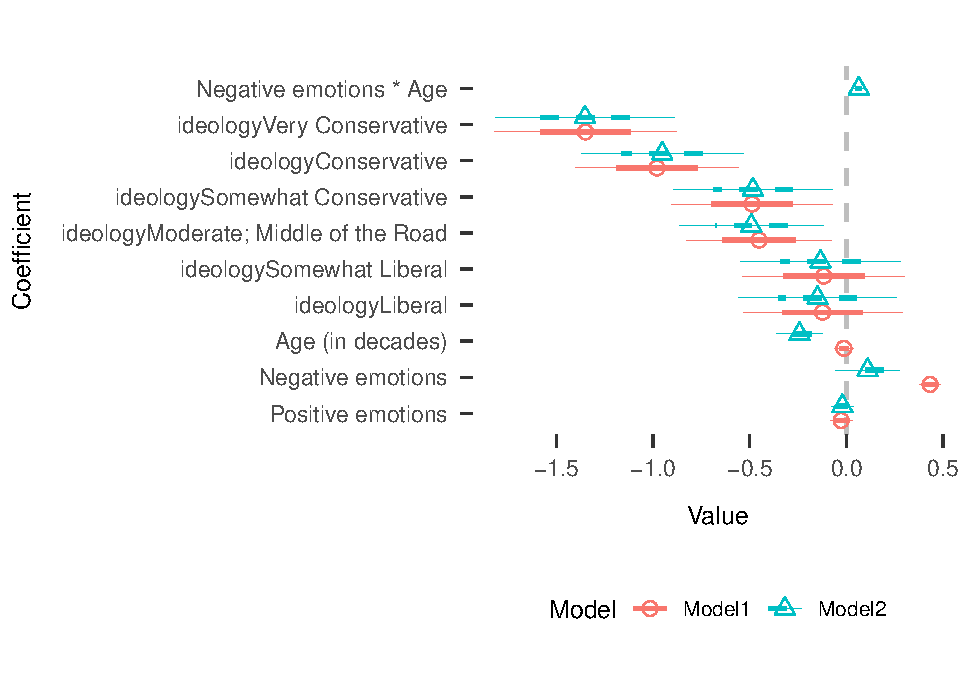
\includegraphics{HelpMyCollaboratorUsesR_files/figure-latex/coefplot-1.pdf}
\caption{\label{fig:coefplot}Unstandardized regression coefficients for a
model without and a model with an interaction effect. The fat and thin
lines represent confidence intervals based on one and two standard
errors.}
\end{figure}

The plot created by \texttt{coefplot} is a \texttt{ggplot2} plot. The
\texttt{ggplot2} package (Wickham et al.,
\protect\hyperlink{ref-R-ggplot2}{2019}) is a versatile, widely used
package. A nice feature of a \texttt{ggplot2}-plot is that we can
customize it further. In the code above, the APA plotting theme from the
\texttt{papaja} package is added and the legend is re-positioned at the
bottom of the figure. The plotting functions in \texttt{coefplot} yield
the data to be plotted instead of a plot if you add the option
\texttt{plot\ =\ FALSE}. With this data set, you can create your own
custom plot with \texttt{ggplot2}.

If you want to have full control of your plots, learn \texttt{ggplot2}.
The book \emph{R for Data Science} (Wickham \& Grolemund,
\protect\hyperlink{ref-WickhamDataScienceImport2017}{2017}) offers a
concise introduction; it is available
\href{https://r4ds.had.co.nz/data-visualisation.html}{online}. The
details of \texttt{ggplot2} can be found in \emph{ggplot2, Elegant
Graphics for Data Analysis} (Wickham,
\protect\hyperlink{ref-wickhamGgplot2ElegantGraphics2009}{2009}), which
has an \href{https://ggplot2-book.org/}{online 3rd edition}.

Plotting regression lines is another appealing way of presenting your
results (Figure \ref{fig:plotregline}). The \texttt{visreg} package
(Breheny \& Burchett, \protect\hyperlink{ref-R-visreg}{2019}) can do
this. It can create \texttt{ggplot2} plots, which can be further
customized. More extensive options are available in the \texttt{effects}
package (Fox, Weisberg, Price, Friendly, \& Hong,
\protect\hyperlink{ref-R-effects}{2019}), but this package cannot
produce \texttt{ggplot2} plots.

\begin{Shaded}
\begin{Highlighting}[]
\CommentTok{# Plot the effect of negative emotions for different age groups.}

\CommentTok{# Load the visreg package.}
\KeywordTok{library}\NormalTok{(visreg)}

\CommentTok{# Create a plot}
\KeywordTok{visreg}\NormalTok{(govact_model2, }
       \DataTypeTok{xvar =} \StringTok{"negemot"}\NormalTok{, }\CommentTok{#variable for the x axis}
       \DataTypeTok{by =} \StringTok{"age"}\NormalTok{, }\CommentTok{#different lines for age groups}
       \DataTypeTok{jitter =} \OtherTok{TRUE}\NormalTok{, }\CommentTok{#negemot has few (discrete) values}
       \DataTypeTok{overlay =} \OtherTok{TRUE}\NormalTok{, }\CommentTok{#show lines in one plot}
       \DataTypeTok{gg =} \OtherTok{TRUE} \CommentTok{#use ggplot2}
\NormalTok{       ) }\OperatorTok{+}
\StringTok{  }\KeywordTok{theme_apa}\NormalTok{() }\OperatorTok{+}\StringTok{ }\CommentTok{#add theme}
\StringTok{  }\CommentTok{#set the axis labels}
\StringTok{  }\KeywordTok{labs}\NormalTok{(}\DataTypeTok{x =} \StringTok{"Negative emotions"}\NormalTok{,}
       \DataTypeTok{y =} \StringTok{"Opinion on government intervention"}\NormalTok{)}
\end{Highlighting}
\end{Shaded}

\begin{figure}[H]
\centering
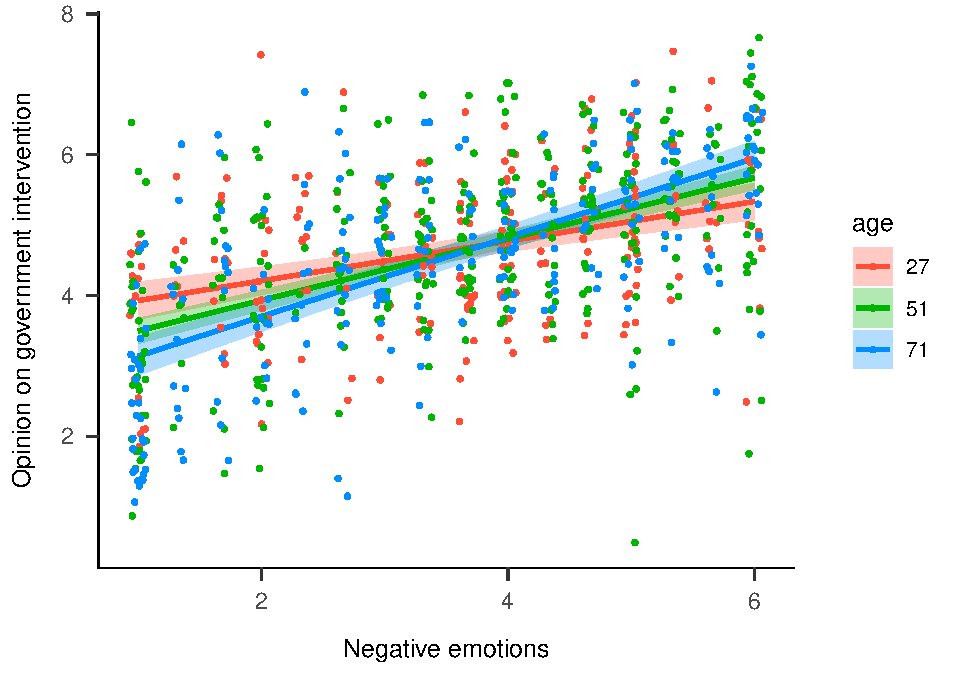
\includegraphics{HelpMyCollaboratorUsesR_files/figure-latex/plotregline-1.pdf}
\caption{\label{fig:plotregline}The effect of negative emotions at different
age levels, 95\% confidence intervals, and partial residuals. Note that
The age groups are defined by default at the 10th, 50th, and 90th
percentiles. Partial residuals have the color of the closest
percentile.}
\end{figure}

Residual plots are commonly used to check regression assumptions. A
fitted regression model contains the residuals. The residuals of the
second regression model estimated in this section are available as
\texttt{govact\_model2\$residuals}.

The \texttt{car} package offers the \texttt{residualPlot()} function to
plot the (unstandardized) residuals against the (unstandardized) fitted
(predicted) values. The related \texttt{residualPlots()} function (note
the plural) also displays the residuals against each of the predictor
variables. Note that these are not \texttt{ggplot} plots. If you are
looking for additional checks and tests for a regression model, consult
the \texttt{car} package.

\begin{Shaded}
\begin{Highlighting}[]
\CommentTok{# Pplot the residuals against the predicted values.}

\CommentTok{# Load package car.}
\KeywordTok{library}\NormalTok{(car)}

\KeywordTok{residualPlot}\NormalTok{(govact_model2,}
             \DataTypeTok{quadratic =} \OtherTok{FALSE}\NormalTok{)}
\end{Highlighting}
\end{Shaded}

\begin{figure}[H]
\centering
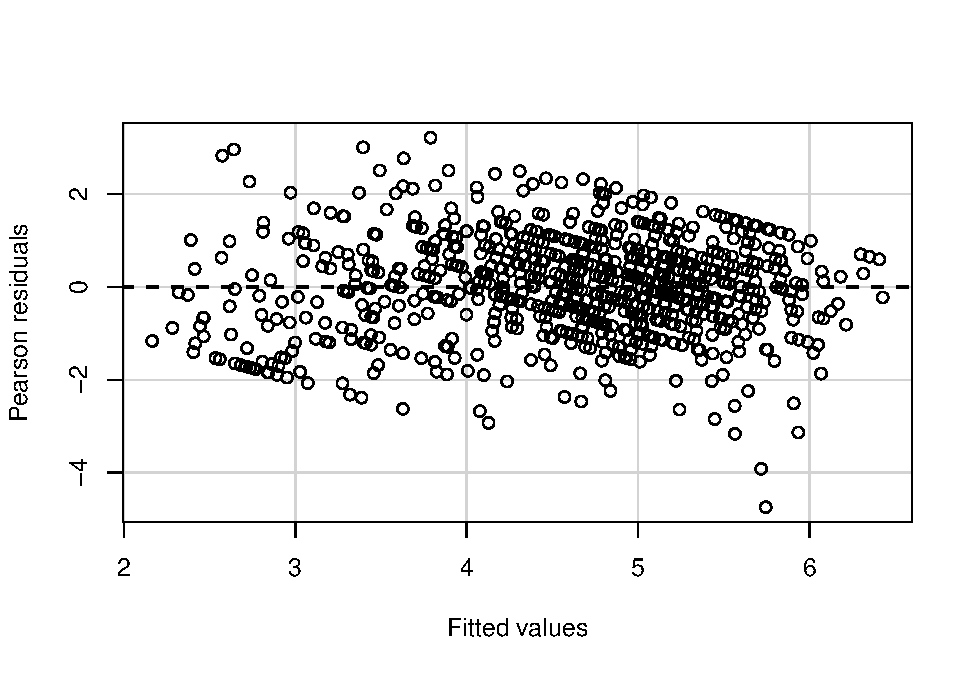
\includegraphics{HelpMyCollaboratorUsesR_files/figure-latex/plotresiduals-1.pdf}
\caption{\label{fig:plotresiduals}A residuals plot for the model predicting
opinion about government intervention from political ideology, positive
emotions, and the interaction between negative emotions and age.}
\end{figure}

\section{Other Common Statistical
Analyses}\label{other-common-statistical-analyses}

R packages offer more statistical analyses than we will probably ever
use. In addition, there can be several packages for the same type of
analysis. The main problem: How do we find the right package?

Volunteers maintain overviews of packages that are dedicated to a
particular task, which are called \emph{task views}. An overview is
available at \url{https://cran.rstudio.com/web/views/}. The
\href{https://cran.rstudio.com/web/views/SocialSciences.html}{SocialSciences}
task view is a good place to start. It reviews packages for estimating
general linear models (regression, analysis of variance) and for
analyzing categorical data.

The most commonly used model types are briefly discussed below in
alphabetical order.

\subsection{Analysis of Variance
(ANOVA)}\label{analysis-of-variance-anova}

The \texttt{aov()} function in the \texttt{stats} package fits an
analysis of variance model. It actually uses the \texttt{lm()} function,
so it can also handle numeric predictors, in which case it offers
analysis of covariance. Apply the \texttt{anova()} function to the
results of \texttt{aov()} or \texttt{lm()} to obtain an ANOVA table with
F tests. If \texttt{anova()} is applied to two or more fitted models,
the F change test is calculated. The models should be nested, otherwise
the F change test does not make sense.

The \texttt{aov()} function uses a \enquote{Type I} test and it should
only be applied to balanced designs. For \enquote{Type II} and
\enquote{Type III} tests or unbalanced designs, use the \texttt{Anova()}
function in the \texttt{car} package. Just like the \texttt{anova()}
function, the model must first be estimated with \texttt{lm()},
\texttt{aov()}, or another linear model.

These functions, as well as \texttt{manova()} in the \texttt{stats}
package, can also be used for multivariate models (more than one
dependent variable) and repeated measures designs.

The \texttt{papaja} package contains several plots for factorial designs
that conform to the APA standard. The \texttt{visreg} package can be
used to visualize results.

\subsection{Chi-squared Tests}\label{chisquared}

A chi-squared test of independence in a contingency table can be
executed with the \texttt{chisq.test()} function in the \texttt{stats}
package. Fisher's exact test is available through the
\texttt{fisher.test()} function in the same package. Both tests require
the specification of two categorical variables with the \texttt{x\ =}
and \texttt{y\ =} arguments.

For example, the following command executes a chi-squared test on the
independence of political ideology and sex in the global warming data
set and stores the result in a data object:

\texttt{fit\_chisq\ \textless{}-\ chisq.test(x\ =\ glbwarm\_spss\$ideology,\ y\ =\ glbwarm\_spss\$sex)}

Note that the data frame must be specified for both variables.

The fitted model is (stored as) a \texttt{htest} object, which includes
both statistical results (chi-squared value, degrees of freedom, and p
value) and the contents of the contingency table: observed frequencies,
expected frequencies under the null hypothesis of independence,
residuals, and standardized residuals. You can inspect the contingency
table by simply sending the list item to the screen, for example,
\texttt{fit\_chisq\$observed} or \texttt{fit\_chisq\$stdres}. The code
below creates an APA6-style contingency table.

\begin{Shaded}
\begin{Highlighting}[]
\CommentTok{# Create a contingency table with observed frequencies and standardized}
\CommentTok{# residuals.}

\CommentTok{# Execute the chi-squared test.}
\NormalTok{fit_chisq <-}\StringTok{ }\KeywordTok{chisq.test}\NormalTok{(}\DataTypeTok{x =}\NormalTok{ glbwarm_spss}\OperatorTok{$}\NormalTok{ideology, }\DataTypeTok{y =}\NormalTok{ glbwarm_spss}\OperatorTok{$}\NormalTok{sex)}

\CommentTok{# Create a table in APA6 style.}
\KeywordTok{data.frame}\NormalTok{( }\CommentTok{#create a data frame from}
    \CommentTok{#residuals matrix added to observed freqs matrix}
    \KeywordTok{cbind}\NormalTok{(fit_chisq}\OperatorTok{$}\NormalTok{observed, fit_chisq}\OperatorTok{$}\NormalTok{stdres)}
\NormalTok{    ) }\OperatorTok\StringTok{ }\CommentTok{#send to next function}
\StringTok{  }\CommentTok{#reorder the columns (variables)}
\StringTok{  }\KeywordTok{select}\NormalTok{(female, female.}\DecValTok{1}\NormalTok{, male, male.}\DecValTok{1}\NormalTok{) }\OperatorTok
\StringTok{  }\CommentTok{#format as table}
\StringTok{  }\KeywordTok{kable}\NormalTok{(}\DataTypeTok{caption =} \StringTok{"Observed frequencies and standardized residuals }
\StringTok{                   for ideology by sex."}\NormalTok{,}
      \DataTypeTok{col.names =} \KeywordTok{rep}\NormalTok{(}\StringTok{""}\NormalTok{, }\DecValTok{4}\NormalTok{), }\CommentTok{#suppress variable names}
      \CommentTok{#the number of digits for all columns}
      \DataTypeTok{digits =} \KeywordTok{c}\NormalTok{(}\DecValTok{0}\NormalTok{, }\DecValTok{2}\NormalTok{, }\DecValTok{0}\NormalTok{, }\DecValTok{2}\NormalTok{), }
      \DataTypeTok{format.args =} \KeywordTok{list}\NormalTok{(}\DataTypeTok{zero.print =} \OtherTok{NULL}\NormalTok{),}
      \DataTypeTok{booktabs =} \OtherTok{TRUE} \CommentTok{#layout with header and bottom lines}
\NormalTok{      ) }\OperatorTok
\StringTok{  }\KeywordTok{kable_styling}\NormalTok{(}
    \CommentTok{#don't move table to top or bottomos a page}
    \DataTypeTok{latex_options =} \KeywordTok{c}\NormalTok{(}\StringTok{"hold_position"}\NormalTok{)}
\NormalTok{  ) }\OperatorTok
\StringTok{  }\CommentTok{#add observed versus standardized residuals header}
\StringTok{  }\KeywordTok{add_header_above}\NormalTok{(}\KeywordTok{c}\NormalTok{(}\StringTok{""}\NormalTok{, }\KeywordTok{rep}\NormalTok{(}\KeywordTok{c}\NormalTok{(}\StringTok{"Observed"}\NormalTok{, }\StringTok{"St.Residual"}\NormalTok{), }\DecValTok{2}\NormalTok{))) }\OperatorTok
\StringTok{  }\CommentTok{#add sex as additional header}
\StringTok{  }\CommentTok{# (2 columns for female, 2 for male)}
\StringTok{  }\KeywordTok{add_header_above}\NormalTok{(}\KeywordTok{c}\NormalTok{(}\StringTok{""}\NormalTok{, }\StringTok{"Female"}\NormalTok{ =}\StringTok{ }\DecValTok{2}\NormalTok{, }\StringTok{"Male"}\NormalTok{ =}\StringTok{ }\DecValTok{2}\NormalTok{)) }\OperatorTok
\StringTok{  }\CommentTok{#footnote with test result, formatted with the papaja::apa_print function}
\StringTok{  }\KeywordTok{footnote}\NormalTok{(}\DataTypeTok{general =} \KeywordTok{paste0}\NormalTok{(}\StringTok{"$Note$. "}\NormalTok{,}
    \KeywordTok{apa_print}\NormalTok{(fit_chisq, }\DataTypeTok{n =} \KeywordTok{sum}\NormalTok{(fit_chisq}\OperatorTok{$}\NormalTok{observed))}\OperatorTok{$}\NormalTok{statistic),}
    \DataTypeTok{general_title =} \StringTok{""} \CommentTok{#suppress standard "Note:"}
\NormalTok{    )}
\end{Highlighting}
\end{Shaded}

\begin{table}[!h]

\caption{\label{tab:chisqtable}Observed frequencies and standardized residuals 
                   for ideology by sex.}
\centering
\begin{tabular}[t]{lrrrr}
\toprule
\multicolumn{1}{c}{} & \multicolumn{2}{c}{Female} & \multicolumn{2}{c}{Male} \\
\cmidrule(l{3pt}r{3pt}){2-3} \cmidrule(l{3pt}r{3pt}){4-5}
\multicolumn{1}{c}{} & \multicolumn{1}{c}{Observed} & \multicolumn{1}{c}{St.Residual} & \multicolumn{1}{c}{Observed} & \multicolumn{1}{c}{St.Residual} \\
\cmidrule(l{3pt}r{3pt}){2-2} \cmidrule(l{3pt}r{3pt}){3-3} \cmidrule(l{3pt}r{3pt}){4-4} \cmidrule(l{3pt}r{3pt}){5-5}
  &  &  &  & \\
\midrule
Very Liberal & 20 & 0.54 & 16 & -0.54\\
Liberal & 64 & 2.03 & 42 & -2.03\\
Somewhat Liberal & 47 & -0.02 & 45 & 0.02\\
Moderate; Middle of the Road & 177 & 2.05 & 141 & -2.05\\
Somewhat Conservative & 47 & -1.10 & 55 & 1.10\\
\addlinespace
Conservative & 45 & -1.82 & 60 & 1.82\\
Very Conservative & 17 & -3.23 & 39 & 3.23\\
\bottomrule
\multicolumn{5}{l}{$Note$. $\chi^2(6, n = 815) = 20.11$, $p = .003$}\\
\end{tabular}
\end{table}

The same functions can be used to apply a one-sample chi-squared test or
goodness-of-fit test. The \texttt{x\ =} argument must specify the
observed frequencies of the categories on the test variable. The
\texttt{base} package function \texttt{table()} does the job. Because
there is no second variable, we do not use the \texttt{y\ =} argument.
Instead, we specify the hypothesized population proportions (argument
\texttt{p\ =}) for the categories. Use the \texttt{c()} function to
combine the proportions and ensure that they are in the right order. For
example, the following code tests the null hypothesis that half of the
population is female and the other half male:

\texttt{fit\_chisq2\ \textless{}-\ chisq.test(x\ =\ table(glbwarm\_spss\$sex),\ p\ =\ c(0.5,\ 0.5))}

The fitted model is stored as a \texttt{htest} object.

\subsection{Regression: Logistic, Poisson, Negative binomial,
Multinomial}\label{glm}

Some regression models for dependent variables that are not numeric and
(in principle) continuous can be estimated with the \texttt{glm()}
function in the \texttt{stats} package. GLM stands for General Linear
Model. The regression model is specified in the same way as the linear
regression model discussed in Section \ref{regressionmodel}. The only
addition is the type of linear predictor and error distribution
(family). The most common families are:

\begin{itemize}
\tightlist
\item
  \texttt{binomial(link\ =\ "logit")} for logistic regression,
\item
  \texttt{poisson(link\ =\ "log")} for Poisson regression,
\item
  \texttt{quasipoisson(link\ =\ "log")} for overdispersed Poisson
  regression.
\end{itemize}

A fitted \texttt{glm()} model is very like a fitted \texttt{lm()} model,
so functions for displaying coefficients (\texttt{coefplot} package) and
fitted regression lines (\texttt{visreg} package) also work for these
models. Thefunctions in the \texttt{car}package such as
\texttt{residualPlot()}, however, only works for linear models.

Negative-binomial regression models can be fit with the
\texttt{glm.nb()} function in the \texttt{MASS} package. This function
follows the same logic as the \texttt{lm()} function for ordinary
regression models. Instead of a model family, you can specify a link
function as an argument. A fitted negative-binomial model has a
structure that is similar to the results of \texttt{lm()} and
\texttt{glm()}. The \texttt{car} and \texttt{coefplot} packages,
however, cannot handle this type of model.

The \texttt{MASS} package also contains a function for ordered logistic
regression, namely \texttt{polr()}. (Unordered) multinomial regression
is provided by the \texttt{multinom()} function in the \texttt{nnet}
package. In both cases, the dependent variable must be a factor.
Logistic, ordered logistic, and multinomial regression with R are
explained in \url{https://rpubs.com/rslbliss/r_logistic_ws}.

\subsection{Regression: Mediation}\label{regression-mediation}

\subsubsection{\texorpdfstring{Package
\texttt{mediation}}{Package mediation}}\label{package-mediation}

For estimating indirect effects in models with one mediator, the
recommended R package is \texttt{mediation} (Tingley et al.,
\protect\hyperlink{ref-R-mediation}{2019}), consult this
\href{https://web.mit.edu/teppei/www/research/mediationR.pdf}{manual}
for more information. This package can handle a continuous outcome
variable in combination with a continuous, ordered, or binary moderator
as well as a binary outcome variable with a continuous or binary
moderator. In all cases, it can handle both continuous and binary
predictors (or treatment variables). In addition, it can control for
continuous and binary covariates.

An important advantage of this package is its ability to perform a
sensitivity test on the indirect (mediated) effect. How sensitive is the
estimated indirect effect to unobserved common causes of the mediator
and the outcome variable? The mediator variable is normally not
randomized, so it can be affected by an unobserved covariate that also
affects the outcome variable. These effects may be incorrectly
attributed to the effect of the mediator on the outcome variable and, as
a consequence, to the indirect effect of the predictor via the mediator
on the outcome.

An unobserved common cause of the mediator and outcome variable would
create a correlation between the residuals in the model predicting the
mediator and the residuals in the model predicting the outcome. The
sensitivity analysis estimates the indirect effect and its confidence
interval for different values of the correlation among the residuals.

A downside to this package is that we have to estimate two regression
models ourselves: one with the mediator as the dependent variable, the
other with the outcome as the dependent variable. This allows us,
however, to report and check the two regression models with the tools
provided in Section \ref{presentingresults}.

Also note that interactions must be included in the regression formula
as separate terms for the conditional and interaction effects, e.g.,
\texttt{y\ \textasciitilde{}\ x1\ +\ x2\ +\ x1:x2} instead of
\texttt{y\ \textasciitilde{}\ x1*x2} and the argument \texttt{INT\ =}
must be set to \texttt{TRUE} in the \texttt{mediate()} function.

\begin{Shaded}
\begin{Highlighting}[]
\CommentTok{# Estimate the indirect effect of sex via negative emotions on opinion about}
\CommentTok{# governmental intervention.}

\CommentTok{# Load the mediation package.}
\KeywordTok{library}\NormalTok{(mediation)}

\CommentTok{# Estimate the regression model for the mediator.}
\NormalTok{fit_mediator <-}\StringTok{ }\KeywordTok{lm}\NormalTok{(negemot }\OperatorTok{~}\StringTok{ }\NormalTok{age }\OperatorTok{+}\StringTok{ }\NormalTok{sex }\OperatorTok{+}\StringTok{ }\NormalTok{ideology, }\DataTypeTok{data =}\NormalTok{ glbwarm_spss) }
\CommentTok{# Estimate the regression model for the outcome.}
\NormalTok{fit_outcome <-}\StringTok{ }\KeywordTok{lm}\NormalTok{(govact }\OperatorTok{~}\StringTok{ }\NormalTok{age }\OperatorTok{+}\StringTok{ }\NormalTok{sex }\OperatorTok{+}\StringTok{ }\NormalTok{ideology }\OperatorTok{+}\StringTok{ }\NormalTok{negemot, }\DataTypeTok{data =}\NormalTok{ glbwarm_spss) }
\CommentTok{# Estimate the indirect effect (may take some time).}
\NormalTok{fit_indirect <-}\StringTok{ }\KeywordTok{mediate}\NormalTok{(fit_mediator, fit_outcome, }\CommentTok{#the two regression models}
                        \DataTypeTok{treat =} \StringTok{"sex"}\NormalTok{, }\CommentTok{#the predictor or treatment variable name}
                        \DataTypeTok{mediator =} \StringTok{"negemot"}\NormalTok{, }\CommentTok{#the mediator name}
                        \DataTypeTok{sims =} \DecValTok{1000}\NormalTok{, }\CommentTok{#number of simulations}
                        \DataTypeTok{boot =} \OtherTok{FALSE} \CommentTok{#use bootstrapping or parametric estimation}
\NormalTok{                        )}
\CommentTok{# Show results:}
\CommentTok{# ACME = Average Causal Mediated Effect (= indirect effect).}
\CommentTok{# ADE = Average Direct Effect.}
\KeywordTok{summary}\NormalTok{(fit_indirect)}
\end{Highlighting}
\end{Shaded}

\begin{verbatim}
## 
## Causal Mediation Analysis 
## 
## Quasi-Bayesian Confidence Intervals
## 
##                Estimate 95% CI Lower 95% CI Upper p-value  
## ACME            -0.0971      -0.1817        -0.01   0.022 *
## ADE             -0.0106      -0.1651         0.15   0.912  
## Total Effect    -0.1077      -0.2816         0.07   0.224  
## Prop. Mediated   0.7455      -5.5105         7.41   0.222  
## ---
## Signif. codes:  0 '***' 0.001 '**' 0.01 '*' 0.05 '.' 0.1 ' ' 1
## 
## Sample Size Used: 815 
## 
## 
## Simulations: 1000
\end{verbatim}

It is more attractive to present the direct and indirect effects in a
diagram. The code below creates a diagram using the \texttt{ggplot2}
package.

\begin{Shaded}
\begin{Highlighting}[]
\CommentTok{# Plot the mediation diagram with ggplot2.}
\CommentTok{# Create coordinates for the variable names.}
\KeywordTok{data.frame}\NormalTok{(}\DataTypeTok{x =} \KeywordTok{c}\NormalTok{(}\FloatTok{0.3}\NormalTok{, }\FloatTok{0.5}\NormalTok{, }\FloatTok{0.7}\NormalTok{), }\CommentTok{#hor. coordinates of labels}
           \DataTypeTok{y =} \KeywordTok{c}\NormalTok{(}\FloatTok{0.1}\NormalTok{, }\FloatTok{0.3}\NormalTok{, }\FloatTok{0.1}\NormalTok{), }\CommentTok{#vert. coordinates of labels}
           \DataTypeTok{hjust =} \KeywordTok{c}\NormalTok{(}\DecValTok{1}\NormalTok{, }\FloatTok{0.5}\NormalTok{, }\DecValTok{0}\NormalTok{),}
           \DataTypeTok{vjust =} \KeywordTok{c}\NormalTok{(}\FloatTok{0.5}\NormalTok{, }\DecValTok{0}\NormalTok{, }\FloatTok{0.5}\NormalTok{),}
           \DataTypeTok{label =} \KeywordTok{c}\NormalTok{(fit_indirect}\OperatorTok{$}\NormalTok{treat, }\CommentTok{#treatment}
\NormalTok{                     fit_indirect}\OperatorTok{$}\NormalTok{mediator, }\CommentTok{#moderator}
                     \StringTok{"govact"}\NormalTok{), }\CommentTok{#outcome variable}
           \CommentTok{# Create start and end coordinates for the arrows}
           \DataTypeTok{xstart =} \KeywordTok{c}\NormalTok{(}\FloatTok{0.3}\NormalTok{, }\FloatTok{0.3}\NormalTok{, }\FloatTok{0.5}\NormalTok{),}
           \DataTypeTok{xend =} \KeywordTok{c}\NormalTok{(}\FloatTok{0.5}\NormalTok{, }\FloatTok{0.7}\NormalTok{, }\FloatTok{0.7}\NormalTok{),}
           \DataTypeTok{ystart =} \KeywordTok{c}\NormalTok{(}\FloatTok{0.1}\NormalTok{, }\FloatTok{0.1}\NormalTok{, }\FloatTok{0.3}\NormalTok{),}
           \DataTypeTok{yend =} \KeywordTok{c}\NormalTok{(}\FloatTok{0.3}\NormalTok{, }\FloatTok{0.1}\NormalTok{, }\FloatTok{0.1}\NormalTok{)}
\NormalTok{           ) }\OperatorTok
\StringTok{  }\CommentTok{#create and show the plot}
\StringTok{  }\KeywordTok{ggplot}\NormalTok{(}\KeywordTok{aes}\NormalTok{(x, y)) }\OperatorTok{+}\StringTok{ }
\StringTok{    }\CommentTok{#arrows}
\StringTok{    }\KeywordTok{geom_segment}\NormalTok{(}\KeywordTok{aes}\NormalTok{(}\DataTypeTok{x =}\NormalTok{ xstart, }\DataTypeTok{y =}\NormalTok{ ystart, }\DataTypeTok{xend =}\NormalTok{ xend, }\DataTypeTok{yend =}\NormalTok{ yend), }
                 \DataTypeTok{arrow =} \KeywordTok{arrow}\NormalTok{(}\DataTypeTok{length =} \KeywordTok{unit}\NormalTok{(}\FloatTok{0.06}\NormalTok{, }\StringTok{"npc"}\NormalTok{), }\DataTypeTok{type =} \StringTok{"closed"}\NormalTok{),}
                 \DataTypeTok{color =} \StringTok{"gray60"}\NormalTok{) }\OperatorTok{+}
\StringTok{    }\CommentTok{#variable names}
\StringTok{    }\KeywordTok{geom_label}\NormalTok{(}\KeywordTok{aes}\NormalTok{(}\DataTypeTok{label=}\NormalTok{label, }\DataTypeTok{hjust =}\NormalTok{ hjust, }\DataTypeTok{vjust =}\NormalTok{ vjust),}
      \DataTypeTok{fill =} \StringTok{"gray60"}\NormalTok{, }\DataTypeTok{color =}\StringTok{"white"}\NormalTok{, }\DataTypeTok{size =} \DecValTok{6}
\NormalTok{      ) }\OperatorTok{+}\StringTok{ }
\StringTok{    }\CommentTok{#direct and indirect effect results}
\StringTok{    }\KeywordTok{geom_text}\NormalTok{(}\KeywordTok{aes}\NormalTok{(}\DataTypeTok{x =} \FloatTok{0.4}\NormalTok{, }\DataTypeTok{y =} \FloatTok{0.2}\NormalTok{, }\DataTypeTok{hjust =} \DecValTok{1}\NormalTok{, }\DataTypeTok{vjust =} \DecValTok{0}\NormalTok{, }\DataTypeTok{label =} \KeywordTok{paste0}\NormalTok{(}\StringTok{"b = "}\NormalTok{, }
                    \KeywordTok{format}\NormalTok{(}\KeywordTok{round}\NormalTok{(fit_mediator}\OperatorTok{$}\NormalTok{coefficients[}\DecValTok{3}\NormalTok{],}\DataTypeTok{digits=}\DecValTok{2}\NormalTok{), }\DataTypeTok{nsmall=}\DecValTok{2}\NormalTok{)))) }\OperatorTok{+}
\StringTok{    }\KeywordTok{geom_text}\NormalTok{(}\KeywordTok{aes}\NormalTok{(}\DataTypeTok{x =} \FloatTok{0.6}\NormalTok{, }\DataTypeTok{y =} \FloatTok{0.2}\NormalTok{, }\DataTypeTok{hjust =} \DecValTok{0}\NormalTok{, }\DataTypeTok{vjust =} \DecValTok{0}\NormalTok{, }\DataTypeTok{label =} \KeywordTok{paste0}\NormalTok{(}\StringTok{"b = "}\NormalTok{, }
                    \KeywordTok{format}\NormalTok{(}\KeywordTok{round}\NormalTok{(fit_outcome}\OperatorTok{$}\NormalTok{coefficients[}\DecValTok{10}\NormalTok{],}\DataTypeTok{digits=}\DecValTok{2}\NormalTok{), }\DataTypeTok{nsmall=}\DecValTok{2}\NormalTok{)))) }\OperatorTok{+}
\StringTok{    }\KeywordTok{geom_text}\NormalTok{(}\KeywordTok{aes}\NormalTok{(}\DataTypeTok{x =} \FloatTok{0.5}\NormalTok{, }\DataTypeTok{y =} \FloatTok{0.11}\NormalTok{, }\DataTypeTok{hjust =} \FloatTok{0.5}\NormalTok{, }\DataTypeTok{vjust =} \DecValTok{0}\NormalTok{,}
      \DataTypeTok{label =} \KeywordTok{paste0}\NormalTok{(}\StringTok{"Direct: b = "}\NormalTok{, }
        \KeywordTok{format}\NormalTok{(}\KeywordTok{round}\NormalTok{(fit_indirect}\OperatorTok{$}\NormalTok{z.avg, }\DataTypeTok{digits =} \DecValTok{2}\NormalTok{), }\DataTypeTok{nsmall =} \DecValTok{2}\NormalTok{), }\StringTok{", 95%CI["}\NormalTok{,}
        \KeywordTok{format}\NormalTok{(}\KeywordTok{round}\NormalTok{(fit_indirect}\OperatorTok{$}\NormalTok{z.avg.ci[[}\DecValTok{1}\NormalTok{]], }\DataTypeTok{digits =} \DecValTok{2}\NormalTok{), }\DataTypeTok{nsmall =} \DecValTok{2}\NormalTok{), }\StringTok{", "}\NormalTok{,}
        \KeywordTok{format}\NormalTok{(}\KeywordTok{round}\NormalTok{(fit_indirect}\OperatorTok{$}\NormalTok{z.avg.ci[[}\DecValTok{2}\NormalTok{]], }\DataTypeTok{digits =} \DecValTok{2}\NormalTok{), }\DataTypeTok{nsmall =} \DecValTok{2}\NormalTok{), }\StringTok{"]"}\NormalTok{))) }\OperatorTok{+}
\StringTok{    }\KeywordTok{geom_text}\NormalTok{(}\KeywordTok{aes}\NormalTok{(}\DataTypeTok{x =} \FloatTok{0.5}\NormalTok{, }\DataTypeTok{y =} \FloatTok{0.09}\NormalTok{, }\DataTypeTok{hjust =} \FloatTok{0.5}\NormalTok{, }\DataTypeTok{vjust =} \DecValTok{1}\NormalTok{,}
      \DataTypeTok{label =} \KeywordTok{paste0}\NormalTok{(}\StringTok{"Indirect: b = "}\NormalTok{, }
        \KeywordTok{format}\NormalTok{(}\KeywordTok{round}\NormalTok{(fit_indirect}\OperatorTok{$}\NormalTok{d.avg, }\DataTypeTok{digits =} \DecValTok{2}\NormalTok{), }\DataTypeTok{nsmall =} \DecValTok{2}\NormalTok{), }\StringTok{", 95%CI["}\NormalTok{,}
        \KeywordTok{format}\NormalTok{(}\KeywordTok{round}\NormalTok{(fit_indirect}\OperatorTok{$}\NormalTok{d.avg.ci[[}\DecValTok{1}\NormalTok{]], }\DataTypeTok{digits =} \DecValTok{2}\NormalTok{), }\DataTypeTok{nsmall =} \DecValTok{2}\NormalTok{), }\StringTok{", "}\NormalTok{,}
        \KeywordTok{format}\NormalTok{(}\KeywordTok{round}\NormalTok{(fit_indirect}\OperatorTok{$}\NormalTok{d.avg.ci[[}\DecValTok{2}\NormalTok{]], }\DataTypeTok{digits =} \DecValTok{2}\NormalTok{), }\DataTypeTok{nsmall =} \DecValTok{2}\NormalTok{), }\StringTok{"]"}\NormalTok{))) }\OperatorTok{+}
\StringTok{    }\KeywordTok{coord_cartesian}\NormalTok{(}\DataTypeTok{xlim =} \KeywordTok{c}\NormalTok{(}\FloatTok{0.2}\NormalTok{, }\FloatTok{0.8}\NormalTok{), }\DataTypeTok{ylim =} \KeywordTok{c}\NormalTok{(}\DecValTok{0}\NormalTok{, }\FloatTok{0.4}\NormalTok{)) }\OperatorTok{+}
\StringTok{    }\KeywordTok{theme_void}\NormalTok{()}
\end{Highlighting}
\end{Shaded}

\begin{figure}[H]
\centering
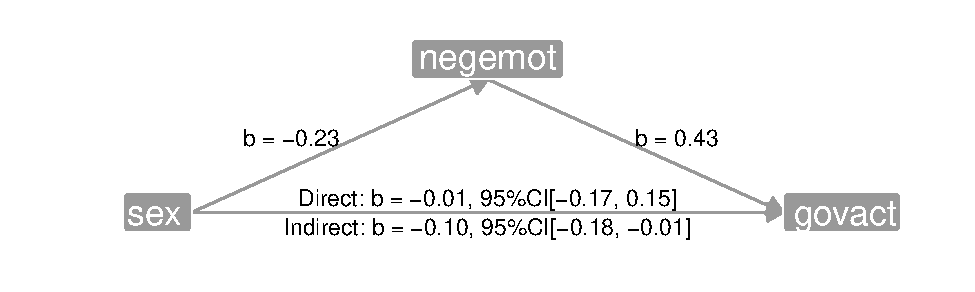
\includegraphics{HelpMyCollaboratorUsesR_files/figure-latex/mediation1plot-1.pdf}
\caption{\label{fig:mediation1plot}Main results of a mediation model
presented as a causal diagram.}
\end{figure}

The sensitivity of the estimated mediation effect to confounders can be
assessed with the \texttt{medsens()} function in the \texttt{mediation}
package. Feed the object with the mediation results to this function
and, if needed, adjust the size of the steps for the residuals
correlation (default = 0.1) that must be checked. See the package
documentation and
\href{https://web.mit.edu/teppei/www/research/mediationR.pdf}{manual}
for more plotting options.

\begin{Shaded}
\begin{Highlighting}[]
\CommentTok{# Execute and plot the sensitivity of the indirect effect to confounders (may}
\CommentTok{# take some time).}
\NormalTok{fit_sens <-}\StringTok{ }\KeywordTok{medsens}\NormalTok{(fit_indirect, }\DataTypeTok{rho.by =} \FloatTok{0.05}\NormalTok{)}

\CommentTok{# Plot the sensitivity results.}
\KeywordTok{plot}\NormalTok{(fit_sens, }\DataTypeTok{sens.par =} \StringTok{"rho"}\NormalTok{)}
\end{Highlighting}
\end{Shaded}

\begin{figure}[H]
\centering
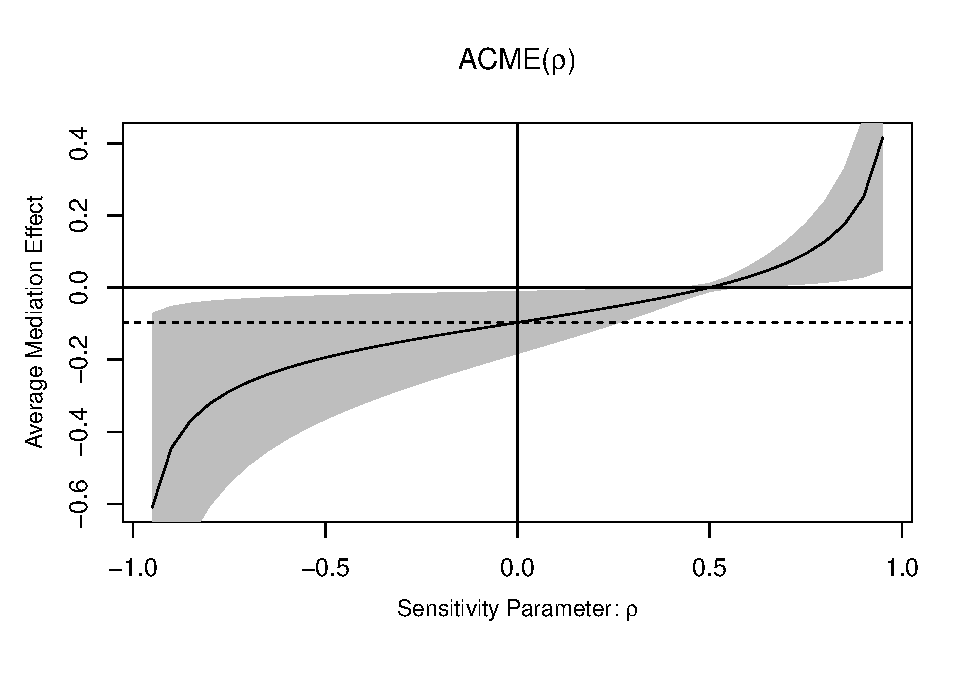
\includegraphics{HelpMyCollaboratorUsesR_files/figure-latex/mediation1sensitivity-1.pdf}
\caption{\label{fig:mediation1sensitivity}The sensitivity of the indirect
effect to confounders.}
\end{figure}

The dashed horizontal line represents the point estimate of the indirect
effect reported above. It is the expected value if the residuals of the
mediator and the residuals of the outcome variable are uncorrelated. In
this case, the estimated indirect effect is not confounded. This point
estimate is a plausible value (namely, within the 95\% confidence
interval) if the correlation between the residuals is negative. This is
the case if the confounder is positively correlated with the mediator
and negatively correlated with the outcome variable or the other way
around.

In contrast, a positive correlation between the residuals decreases the
size of the negative indirect effect and turns it into a positive effect
around a correlation of 0.5. Around a correlation of 0.40 (see
\texttt{summary(fit\_sens)} for the exact number), zero is included in
the confidence interval. For correlations above 0.40, we are no longer
confident that the indirect effect is negative. A correlation of this
size between the residuals requires a confounder that is strongly
correlated (above 0.60) with both the mediator and the outcome variable
(0.60 * 0.60 = 0.36). If we can't think of such a confounder, we can be
quite confident that the indirect effect is negative.

\subsubsection{\texorpdfstring{Package
\texttt{psych}}{Package psych}}\label{package-psych}

As an alternative, the \texttt{psych} package (Revelle,
\protect\hyperlink{ref-R-psych}{2019}) also offers a \texttt{mediate()}
function to estimate a mediation model. It handles models with a single
mediator and models with parallel mediation: two or more mediators
without effects between mediators. Like the PROCESS macro for SPSS (A.
F. Hayes,
\protect\hyperlink{ref-HayesIntroductionMediationModeration2013}{2013}),
the \texttt{psych::mediat()} function performs all regression analyses
in one go and it uses bootstrapping to estimate the confidence interval
of the indirect effect.

This function automatically plots the results as a causal diagram. It
cannot handle factors, so you have to replace them by 0/1 variables
beforehand. The following code shows how to create a dichotomous
variable \texttt{female} (0 = no, 1 = yes) fom the factor \texttt{sex}
in \texttt{glbwarm\_spss} (using the \texttt{tidyverse} function
\texttt{mutate()}):

\texttt{glbwarm\_spss\ \textless{}-\ mutate(glbwarm\_spss,\ female\ =\ ifelse(sex\ ==\ \textquotesingle{}female\textquotesingle{},\ 1,\ 0))}

More complicated mediation models can be estimated with packages for
structural equation modelling (Section \ref{sem}).

\subsection{Regression: Moderation}\label{regression-moderation}

Moderation in linear regression analysis is exemplified in Section
\ref{customtables}. This approach also applies to other types of
regression models (Section \ref{glm}).

Mean-centering of predictor or moderator variables is relatively easy,
because we directly get the mean of a variable with the \texttt{mean()}
function.

\begin{Shaded}
\begin{Highlighting}[]
\CommentTok{# Mean-centering in basic R (ignoring missing values.}
\NormalTok{dataset}\OperatorTok{$}\NormalTok{newvariable <-}\StringTok{ }\NormalTok{dataset}\OperatorTok{$}\NormalTok{variable }\OperatorTok{-}\StringTok{ }\KeywordTok{mean}\NormalTok{(dataset}\OperatorTok{$}\NormalTok{variable, }\DataTypeTok{na.rm =} \OtherTok{TRUE}\NormalTok{)}
\CommentTok{# Mean-centering with tidyverse (ignoring missing values.}
\NormalTok{dataset <-}\StringTok{ }\NormalTok{dataset }\OperatorTok
\StringTok{  }\KeywordTok{mutate}\NormalTok{(}\DataTypeTok{newvariable =}\NormalTok{ variable }\OperatorTok{-}\StringTok{ }\KeywordTok{mean}\NormalTok{(dataset}\OperatorTok{$}\NormalTok{variable, }\DataTypeTok{na.rm =} \OtherTok{TRUE}\NormalTok{))}
\CommentTok{# Mean-centering within a regression formula (ignoring missing values.}
\NormalTok{fit <-}\StringTok{ }\KeywordTok{lm}\NormalTok{(y }\OperatorTok{~}\StringTok{ }\KeywordTok{I}\NormalTok{(variable }\OperatorTok{-}\StringTok{ }\KeywordTok{mean}\NormalTok{(dataset}\OperatorTok{$}\NormalTok{variable, }\DataTypeTok{na.rm =} \OtherTok{TRUE}\NormalTok{))}\OperatorTok{*}\NormalTok{anothervariable)}
\end{Highlighting}
\end{Shaded}

\subsection{Regression: Multilevel}\label{regression-multilevel}

Multilevel models can be estimated with the the \texttt{nlme} package
(Pinheiro, Bates, \& R-core, \protect\hyperlink{ref-R-nlme}{2019}) or
\texttt{lme4} (Bates, Maechler, Bolker, \& Walker,
\protect\hyperlink{ref-R-lme4}{2019}). The first package allows for
autocorrelated or heteroscedastic individual-level errors whereas the
second package supports cross-nested random effects.

In the functions of the \texttt{nlme}package, \texttt{lme()} for linear
models and \texttt{nlme()} for non-linear models, the fixed effects of
the model are specified with a formula in the usual way. In addition,
the \texttt{random\ =} argument specifies effects that vary at a higher
level.

The functions \texttt{lmer()} and \texttt{glmer()} in the \texttt{lme4}
package estimate multilevel models for linear and generalized linear
models respectively. Random effects are added to the model formula using
a vertical bar (\texttt{\textbar{}}). For example,
\texttt{(1\ \textbar{}\ subject)} adds random intercepts at the subject
level, while \texttt{(1\ +\ age\ \textbar{}\ subject)} adds varying
intercepts and varying slopes for age at the subject level as well as a
covariance between the random intercepts and slopes. Note that
\texttt{subject} must be the name of a variable identifying subjects as
higher level units.

Non-linear multilevel models, for example, multilevel logistic
regression models, are notably hard to estimate. For this type of
models, a Bayesian approach with MCMC estimation is usually preferred.
The \texttt{rstanarm} package (Gabry \& Goodrich,
\protect\hyperlink{ref-R-rstanarm}{2019}) contains functions that have
the same structure and the same type of output as the multilevel
functions in the \texttt{lme4} package.

\subsection{Structural Equation Modelling}\label{sem}

The \texttt{lavaan} package (Rosseel \& Jorgensen,
\protect\hyperlink{ref-R-lavaan}{2019}) for structural equation
modelling was created and is maintained by an active
\href{http://lavaan.ugent.be/}{research group} specialized in structural
equation modelling. Recent developments include multilevel SEMs and
Bayesian approaches.\texttt{OpenMx} is another SEM package (Boker et
al., \protect\hyperlink{ref-R-OpenMx}{2019}) for R that is actively
developed. A third popular SEM package in R is \texttt{sem}.

In all packages, a model must be specified (typed) as a set of
structural equations, which are similar to regression formulas.
Standalone free software (\href{http://onyx.brandmaier.de/}{Onyx}) is
available in which a structural equation model can be drawn and the
resulting \texttt{lavaan} or \texttt{OpenMx} model code can be saved and
used in R. In addition, Onyx can read and visualize models created in
\texttt{OpenMx}. The \texttt{semPlot} package can create diagrams from
lavaan results.

For more information, consult the
\href{https://cran.r-project.org/web/views/Psychometrics.html}{Psychometric
Models and Methods} task view.

\subsection{t Tests}\label{ttests}

It is possible to use the R function for linear (regression) models
(\texttt{lm()}) to execute one-sample, paired-samples, and
independent-samples t tests. The \texttt{stats} package also contains
the \texttt{t.test()} function for this purpose. This function offers
the option to set the test value (also for the mean difference in a
paired-samples or independent-samples t test), the direction of the test
(left-sided, right-sided, and two-sided), and the confidence level.
Another advantage of the \texttt{t.test()} function is that it yields a
results object of class \texttt{htest}, which can be summarized in APA6
format with the \texttt{apa\_print()} function in the \texttt{papaja}
package (see Section \ref{inlineAPA}). The code below exemplifies a
right-sided one-sample t test.

\begin{Shaded}
\begin{Highlighting}[]
\CommentTok{# Right-sided, one-sample t-test with 4.0 as hypothesized population value.}
\NormalTok{one_sample <-}\StringTok{ }\KeywordTok{t.test}\NormalTok{(}
  \DataTypeTok{x =}\NormalTok{ glbwarm_spss}\OperatorTok{$}\NormalTok{govact, }\CommentTok{#test variable}
  \DataTypeTok{mu =} \FloatTok{4.0}\NormalTok{, }\CommentTok{#test value}
  \DataTypeTok{alternative =} \StringTok{"greater"}\NormalTok{, }\CommentTok{#"two.sided" (default), "greater" or "less"}
  \DataTypeTok{conf.level =} \FloatTok{0.95} \CommentTok{#confidence level}
\NormalTok{)}
\CommentTok{# Have a look at the contents of results object one_sample.}
\end{Highlighting}
\end{Shaded}

Note that the command does not have a \texttt{data\ =} argument, like
\texttt{lm()}, so you have to supply the name of the data frame with the
variable(s) that you use in the test. In addition, one-sided tests yield
a confidence interval with plus or minus infinity (\texttt{Inf} or
\texttt{-Inf}) as one of the boundaries.

A paired-samples t test is quite straightforward: just add a second
variable with the \texttt{y\ =} argument and set the \texttt{paired\ =}
argument to \texttt{TRUE} (see the code below). An independent-samples t
test is a bit more complicated. First, we have to determine if the two
groups have equal population variances because this affects the way the
standard error must be calculated. We can do this with the
\texttt{var.test()} function in the \texttt{stats} package. In the code
below, we use the \texttt{p.value} of this test in the
\texttt{var.equal\ =} argument of the t test. The code
\texttt{(result\_var\$p.value\ \textgreater{}\ 0.05)} returns
\texttt{TRUE} if the equal variances test is not significant at the .05
level (the p value is above .05) and it returns \texttt{FALSE}
otherwise. Instead of telling the t test manually whether the equal
variances assumption is true or false, we let the results of the equal
variances test provide this information. This way, we are sure that the
right option is selected.

\begin{Shaded}
\begin{Highlighting}[]
\CommentTok{# Two-sided paired samples t test: Average difference between positive and}
\CommentTok{# negative emotions is zero in the population (nonsensical example).}
\NormalTok{paired_samples <-}\StringTok{ }\KeywordTok{t.test}\NormalTok{(}
  \DataTypeTok{x =}\NormalTok{ glbwarm_spss}\OperatorTok{$}\NormalTok{posemot,}
  \DataTypeTok{y =}\NormalTok{ glbwarm_spss}\OperatorTok{$}\NormalTok{negemot,}
  \DataTypeTok{paired =} \OtherTok{TRUE}\NormalTok{,}
  \DataTypeTok{mu =} \DecValTok{0} \CommentTok{#hypothesized difference x - y}
\NormalTok{)}

\CommentTok{# One-sided independent-samples t test: Do females score on average 1.0 higher}
\CommentTok{# than males in their opinion on government intervention?}
\CommentTok{# First: test on equal variances (in stat package).}
\NormalTok{result_var <-}\StringTok{ }\KeywordTok{var.test}\NormalTok{(govact }\OperatorTok{~}\StringTok{ }\NormalTok{sex, }\DataTypeTok{data =}\NormalTok{ glbwarm_spss)}
\CommentTok{# Second: t-test using the equal variances test result.}
\NormalTok{indep_samples <-}\StringTok{ }\KeywordTok{t.test}\NormalTok{(}
\NormalTok{  govact }\OperatorTok{~}\StringTok{ }\NormalTok{sex, }\CommentTok{#lm() formula!}
  \DataTypeTok{data =}\NormalTok{ glbwarm_spss, }\CommentTok{#works only with a formula}
  \DataTypeTok{mu =} \FloatTok{1.0}\NormalTok{, }\CommentTok{#test value: females are second category}
  \DataTypeTok{paired =} \OtherTok{FALSE}\NormalTok{, }\CommentTok{#not a paired t test}
  \DataTypeTok{var.equal =}\NormalTok{ (result_var}\OperatorTok{$}\NormalTok{p.value }\OperatorTok{>}\StringTok{ }\FloatTok{0.05}\NormalTok{), }\CommentTok{#equal variances?}
  \DataTypeTok{alternative =} \StringTok{"less"} \CommentTok{#males are coded 2 (or 1), females 1 (or 0)}
\NormalTok{)}
\end{Highlighting}
\end{Shaded}

\subsection{Time Series Analysis}\label{time-series-analysis}

The
\href{https://cran.r-project.org/web/views/TimeSeries.html}{TimeSeries
task view} presents a large variety of packages and functions for time
series analysis in R. The packages assume that you have your dates and
times correct in your R data set. Dates and times are notoriously
troublesome because they are complicated (leap years, time zones,
\ldots{}) and there are different conventions for storing dates and
times on computers. I recommend to use the \texttt{lubridate} package
(Spinu, Grolemund, \& Wickham,
\protect\hyperlink{ref-R-lubridate}{2018}) for reading and manipulating
dates and times. See the
\href{https://r4ds.had.co.nz/dates-and-times.html}{chapter on dates and
times} in \emph{R for Data Science} (Wickham \& Grolemund,
\protect\hyperlink{ref-WickhamDataScienceImport2017}{2017}) for more
information.

\begin{quote}
Check: Always compare some dates/times in your R data set to your
original data set.
\end{quote}

\section{Reproducible Analyses With R Markdown}\label{rmarkdown}

The document that you are reading at this moment was created in R. It
contains both the text that you are reading and the R code analyzing the
data and creating the tables and plots displaying the results. The
document is written in R Markdown, a relatively simple text processor. R
Markdown documents can be rendered into PDF (LaTeX), HTML, and sometimes
Word documents.

Anyone who has the R Markdown document and the data sets used in it can
reproduce the results as well as the results tables and plots. Every
step in the analysis process and every report detail can be checked and,
where necessary, criticized and improved. Mastering R and understanding
the structure of an R Markdown document makes the analyses and report
fully transparent.

\subsection{Integrating Text and Code}\label{integratingtextcode}

Download the R Markdown document
\href{https://wdenooy.github.io/Switch2R/HelpMyCollaboratorUsesR.Rmd}{HelpMyCollaboratorUsesR.Rmd}
that generates the document you are now reading, save it to your current
R project directory, and open it in RStudio to see an example. The
document illustrates many features of R Markdown, so you may use it as a
reference for your own work. If you see a feature in the
\href{https://wdenooy.github.io/Switch2R/HelpMyCollaboratorUsesR.pdf}{PDF}
or web version of the document that you want to use, check the R
Markdown document to find out how it is done.

\subsubsection{Code chunks}\label{code-chunks}

\begin{figure}[h]
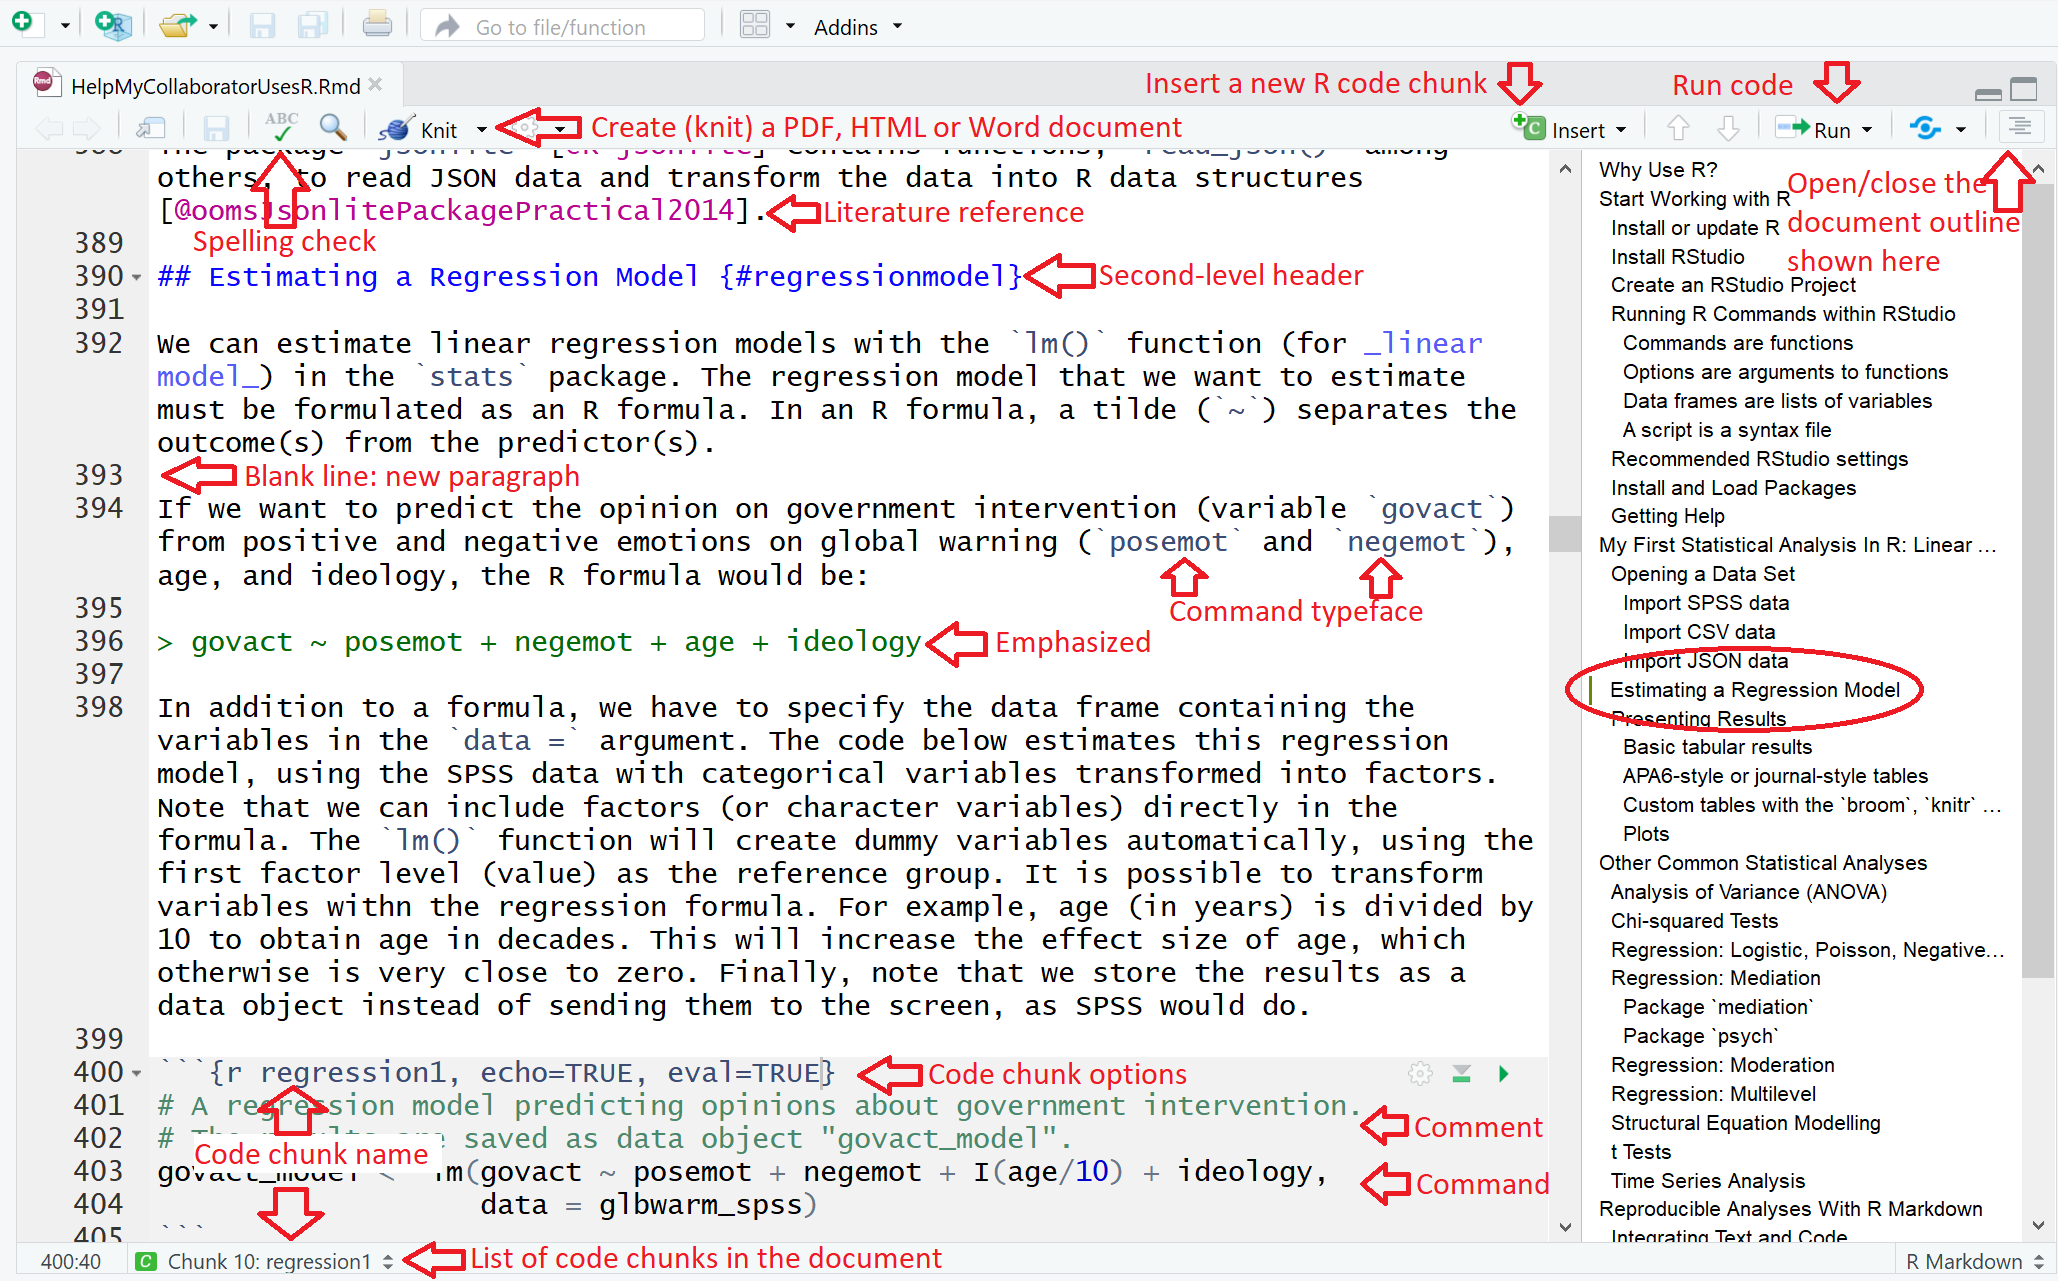
\includegraphics[width=6.86in]{RMarkdown} \caption{Part of the R Markdown document HelpMyCollaboratorUsesR.Rmd.}\label{fig:RMarkdown}
\end{figure}

Figure \ref{fig:RMarkdown} shows a small part of the R Markdown document
that generates the current document. Several noteworthy features are
marked. Let us focus on the way R code is incorporated in the document.
At line 400, a code chunk starts, which has a grey background. Commands
and comments can be included in a code chunk just like they are included
in a script file (Section \ref{scriptfile}).

A code chunk starts with a header (in between \texttt{\{\}}). The header
starts with the letter \texttt{r} indicating that the code chunk
contains R code; it can also contain python and other types of code.
Then, an optional name is given to the code chunk. Names show up in the
outline of code chunks (the drop-down list in the bottom-left of the R
Markdown window), so an informative name helps to quickly locate the
code chunk later on.

In addition there are several options for the code chunk, two of which
are shown here. The option \texttt{echo=} determines whether
(\texttt{TRUE}) or not (\texttt{FALSE}) the code will be shown in the
output document. Normally, we hide code but the current document shows
most of the code for learning purposes. The option \texttt{eval=}
determines whether (\texttt{TRUE}) or not (\texttt{FALSE}) the code will
be executed. Usually, we want to execute the code. For more information,
see \url{https://yihui.name/knitr/options/\#chunk-options}.

Do not economize on comments within code chunks. They allow you to
incorporate your thoughts about the R code in the R markdown document.
Thus, you can document why you do what you do, which approaches you
tried that did not work (and why), what remains to be done, and so on.

The R Markdown document is created (knitted) line by line from the start
to the end. Code chunks are executed when they are encountered in this
process. A data set opened in a code chunk or a results object created
in a code chunk are available to later code chunks but not to previous
code chunks.

\subsubsection{Inline APA6-style statistical results}\label{inlineAPA}

Code and text can be integrated even more tightly. R functions can be
embedded within sentences, so code results become part of the sentence.
We can pull the mean and standard deviation of the opinion about
government intervention for males from the data frame with the following
code (using the \texttt{printnum()} function in \texttt{papaja}):

\begin{Shaded}
\begin{Highlighting}[]
\CommentTok{# R code for inline use within a sentence.}
\StringTok{`}\DataTypeTok{r printnum(mean(glbwarm_spss$govact[glbwarm_spss$sex == "male"]))}\StringTok{`}
\StringTok{`}\DataTypeTok{r printnum(sd(glbwarm_spss$govact[glbwarm_spss$sex == "male"]))}\StringTok{`}
\end{Highlighting}
\end{Shaded}

Pay attention to the special quotation marks and the \texttt{r}
indicating that we are dealing with R code. Without the quotation marks
and \texttt{r} letter, the code will not work. If we include this code
in a sentence, we get the following result:

Males are on average less positive about government action (\emph{M} =
4.45, \emph{SD} = 1.53 than females (\emph{M} = 4.72, \emph{SD} = 1.16).

Note that the numbers are pulled directly from the data set, so we
cannot make mistakes by typing errors. In addition, if we discover and
correct a mistake in the data, re-creating the output document will
ensure that the new results are shown in the text.

The \texttt{papaja} package also contains functions that extract
relevant statistical results from a results object and format them
according to the APA6 guidelines. The following command formats the
results of the independent-samples t test from Section \ref{ttests},
which we stored in the object \texttt{indep\_samples}:

\begin{Shaded}
\begin{Highlighting}[]
\StringTok{`}\DataTypeTok{r apa_print(indep_samples)$full_result}\StringTok{`}
\end{Highlighting}
\end{Shaded}

Embedded within a sentence: This difference is statistically
significant, \(\Delta M = 0.27\), 95\% CI \([-\infty\), \(0.43]\),
\(t(741.55) = -7.66\), \(p < .001\).

\subsubsection{Cross-references and literature
references}\label{crossreferences}

R Markdown by itself does not support cross-references to sections,
tables, figures, or equations. The \texttt{bookdown} package (Xie,
\protect\hyperlink{ref-R-bookdown}{2019}\protect\hyperlink{ref-R-bookdown}{a})
adds these features. This is not an ordinary package that you load with
the \texttt{library()} function. It must be used when the R Markdown
document is knitted into the output document. This happens automatically
when you use the APA6 journal article template as your starting point
for a new R Markdown document (see Section \ref{apa6template}).

With the \texttt{bookdown} package in place, you can reference a table
or figure using the name of the code chunk that creates the table or
figure. For example, \texttt{\textbackslash{}@ref(tab:papajatable)}
would insert the number of the table created with \texttt{papaja} in
Section \ref{APAtables} in the text, because the code chunk creating
this table is named \texttt{papajatable}(check the R Markdown document
to see this). Similarly, \texttt{\textbackslash{}@ref(fig:coefplot)}adds
the number of the figure with the plotted regression coefficients in
Section \ref{plots}. Note the \texttt{tab:} and \texttt{fig:} parts,
which are mandatory for references to tables and figures.

If you want to cross-reference a section, you have to add a label to the
section header, for example, \texttt{\{\#crossreferences\}} for the
present section. Now, \texttt{\textbackslash{}@ref(crossreferences)}
inserts the number of this section in a sentence, for example, this is a
reference to Section \ref{crossreferences}.

References to literature are best created from a BibTeX database. In a
BibTeX database, each entry has an identifier, for
example,\texttt{WickhamDataScienceImport2017} could be the identifier of
the \emph{R for Data Science} book. In the top of the R Markdown
document (also called the YAML front matter), the name of your
BibTeX-file should be mentioned in the \texttt{bibliography:} field. See
the R Markdown document
\href{https://wdenooy.github.io/Switch2R/HelpMyCollaboratorUsesR.Rmd}{\emph{HelpMyCollaboratorUsesR.Rmd}}
for an example.

To include a reference to this book, add
\texttt{{[}@WickhamDataScienceImport2017{]}} in your sentence. The
square brackets \texttt{{[}{]}} will be replaced by parentheses. Omit
the brackets if you do not want to have parentheses. If you do not want
to show the author names, put a minus sign before \texttt{@}. You can
add text within the brackets, for example:
\texttt{{[}see\ @WickhamDataScienceImport2017:\ 211{]}}.

It is a bit of a hassle to create a BibTeX file with all references and
using the IDs from this file to add references to literature in your R
Markdown text. The RStudio add-in \texttt{citr} makes this a lot easier,
especially if you store your literature in Zotero (see
\url{https://github.com/crsh/citr}). For more information, read the
concise and handy book \emph{Bookdown. Authoring Books and Technical
Documents with R Markdown} (Xie,
\protect\hyperlink{ref-xieBookdownAuthoringBooks2016}{2016}), which is
also available
\href{https://bookdown.org/yihui/bookdown/citations.html}{online}.

When you knit the document, a list of references will be added
automatically, containing all literature referred to in the text. This
requires some settings in your R Markdown file, which won't be discussed
here (see, for example,
\url{https://rmarkdown.rstudio.com/authoring_bibliographies_and_citations.html})
because they are standard provided in the APA6 R Markdown template,
which we recommend to use. Let us turn to this template now.

\subsection{APA6 Journal Article Template}\label{apa6template}

\begin{wrapfigure}{r}{0.45\textwidth}
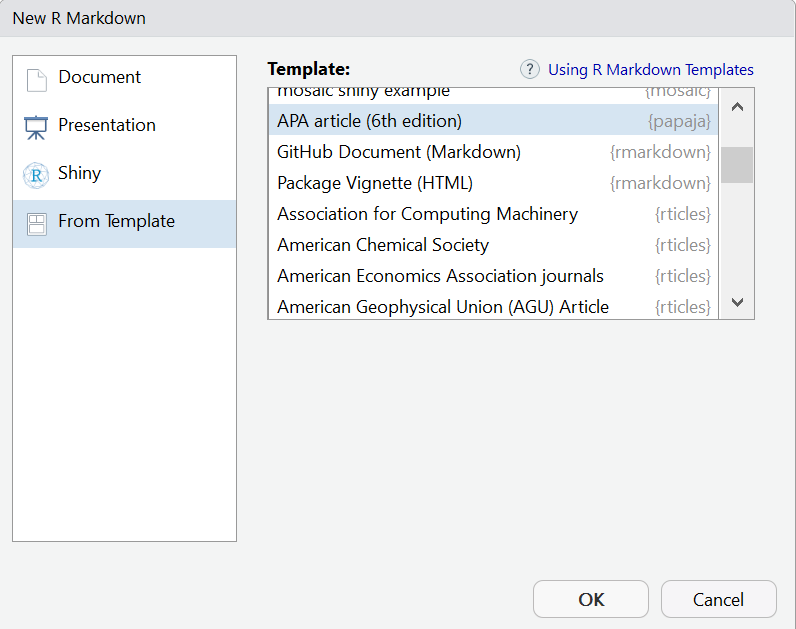
\includegraphics[width=2.65in]{template} \caption{R Markdown templates dialog box.}\label{fig:template}
\end{wrapfigure}

The \texttt{papaja} package contains a template for an APA6-style
journal article. Once \texttt{papaja} is installed, you can select the
APA template when creating a new Markdown file through the RStudio menu:
Select \emph{File}, \emph{New File}, \emph{R Markdown} and in the dialog
box (Figure \ref{fig:template}), select \emph{From Template} and
\emph{APA Article (6th edition)}.

Browse through the R Markdown document of this template. You can add
author names and affiliations, an abstract, keywords, line numbers, and
so on. Not all information will be nicely rendered in HTML output but it
should be in PDF.

\subsection{Creating a HTML, PDF, and Word
Document}\label{creating-a-html-pdf-and-word-document}

The R Markdown document is great for sharing with your collaborators
because they can check all your work and add their own work. Especially
in the code chunks, use comments a lot to explain to your collaborators
and to yourself the purpose of the code.

The R Markdown document, however, is not meant for the general reader or
for publication (although it would be great to add it as online
materials to a publication). For the general reader and publication, the
R Markdown document must be rendered (\enquote{knitted}) into HTML for
web publication and PDF for paper printing (and journal submission). It
is usually better to render the document as HTML first because this is
much faster than rendering a PDF. You can spot errors and typos quickly
in the HTML version and correct them before you render into PDF.

Rendering to PDF requires a LaTeX installation on your computer. RStudio
refers you to the websites where you can download and install LaTeX for
your type of computer when you try to render to PDF without a LaTeX
installation. Downloading may take some time, especially for Mac
computers. Make sure that you have a fast and stable internet
connection.

Rendering to PDF proceeds in several steps with a TeX file as one of the
intermediate steps. The APA template saves the intermediary TeX file,
which can be edited in (free) software like
\href{https://www.xm1math.net/texmaker/}{Texmaker} or online
applications such as \href{https://www.overleaf.com/}{Overleaf}. In my
experience, there are always some technical and layout problems to be
solved before the PDF output is fully satisfactory. For example, a table
footnote created with \texttt{kableExtra} escapes the special character
\texttt{\$} for math symbols by adding a \texttt{\textbackslash{}}
before it. The combination \texttt{\textbackslash{}\$} in table notes
must be replaced by \texttt{\$} in the TeX file.

A Word document can also be created from the APA template but this
option is marked as experimental, so we should not expect everything to
render correctly. It can be more efficient to open the rendered HTML or
PDF in Word, if you need a Word document.

\section{And More \ldots{}}\label{and-more}

Finally, some pointers to additional R skills.

\subsection{Data Wrangling: Preparing and Cleaning your
Data}\label{data-wrangling-preparing-and-cleaning-your-data}

Apart from incidental recoding of values and custom table construction,
this paper does not discuss data management. For reproducible analyses,
data cleaning should be part of the R Markdown document. Unfortunately,
data management is a vast territory that cannot be summarized here.

For those who want to dive into this subject, I recommend the tidyverse
approach as presented in the book \emph{R for Data Science} (Wickham \&
Grolemund, \protect\hyperlink{ref-WickhamDataScienceImport2017}{2017}),
in particular Chapters 3 and 9-14. Chapter 3 of
\href{https://moderndive.com/index.html}{\emph{ModernDive: An
Introduction to Statistical and Data Sciences via R}} (Ismay \& Kim,
\protect\hyperlink{ref-IsmayIntroductionStatisticalData}{2019}) offers a
more concise introduction.

\subsection{Downloading Data from the
Web}\label{downloading-data-from-the-web}

There are packages for scraping web data, for example \texttt{rvest}
(Wickham,
\protect\hyperlink{ref-R-rvest}{2019}\protect\hyperlink{ref-R-rvest}{b})
and \texttt{httr}(Wickham,
\protect\hyperlink{ref-R-httr}{2019}\protect\hyperlink{ref-R-httr}{a}).
See, for example, this
\href{https://www.datacamp.com/courses/working-with-web-data-in-r}{DataCamp}
course.

\subsection{Writing Your Own
Functions}\label{writing-your-own-functions}

R is a set of functions. It is easy to write your own functions, see
Chapter 15 in \emph{R for Data Science} (Wickham \& Grolemund,
\protect\hyperlink{ref-WickhamDataScienceImport2017}{2017}). The code
below shows the general template for creating a new function.

\begin{Shaded}
\begin{Highlighting}[]
\CommentTok{# Function template:}
\NormalTok{new_function_name <-}\StringTok{ }\ControlFlowTok{function}\NormalTok{ (argument1, }\DataTypeTok{argument2 =} \DecValTok{0}\NormalTok{) \{}
  
  \CommentTok{#your code}
  
  \KeywordTok{return}\NormalTok{(what_you_want_to_return) }
  \CommentTok{#or just return the last thing}
\NormalTok{\}}
\end{Highlighting}
\end{Shaded}

\subsection{Collaborating via Github}\label{collaborating-via-github}

If you are part of a team working on the same research project, you
would like to have an easy way of working with several people on the
same R Markdown document. What changes and additions do your
collaborators make to the document and how do they comment on your work?
If at some point mistakes have been introduced, can we roll back to a
previous version?

Version control software combined with a cloud repository offers an
answer to these questions. \emph{Git} is popular version control
software and \emph{Github} is a cloud repository designed for working
with Git. RStudio projects can be linked to Git and Github, see
\href{https://support.rstudio.com/hc/en-us/articles/200532077}{Using
Version Control with RStudio} and links on that page for details (a good
resource is \href{http://happygitwithr.com/}{Happy Git and Github for
the useR}). This document uses Git and
\href{https://github.com/WdeNooy/Switch2R}{Github}.

Once an RStudio project is linked to Git, the top-right panel in the
RStudio interface contains a \emph{Git} tab for easy synchronization of
the local R Markdown document that you are working on and the remote
document in the cloud (Github repository) that is accessible to all
collaborators.

\begin{enumerate}
\def\labelenumi{\arabic{enumi}.}
\item
  When you start working on a file, download (\emph{Pull}) the latest
  version from the repository, so you are working on the latest version.
  The file(s) from the repository will replace your local file(s).
\item
  When you are ready, upload your local version to the repository.
  First, \emph{Commit} the changes that you made to the file. This will
  make Git register a new version of the file and remember the changes
  that you made. Second, upload (\emph{Push}) your changed version to
  the cloud repository (Github).
\end{enumerate}

RStudio also supports another version control software: Subversion.

\newpage

\section{References}\label{references}

\begingroup
\setlength{\parindent}{-0.5in} \setlength{\leftskip}{0.5in}

\hypertarget{refs}{}
\hypertarget{ref-R-papaja}{}
Aust, F., \& Barth, M. (2019). \emph{Papaja: Prepare reproducible apa
journal articles with r markdown}. Retrieved from
\url{https://github.com/crsh/papaja}

\hypertarget{ref-R-lme4}{}
Bates, D., Maechler, M., Bolker, B., \& Walker, S. (2019). \emph{Lme4:
Linear mixed-effects models using 'eigen' and s4}. Retrieved from
\url{https://CRAN.R-project.org/package=lme4}

\hypertarget{ref-R-OpenMx}{}
Boker, S. M., Neale, M. C., Maes, H. H., Spiegel, M., Brick, T. R.,
Estabrook, R., \ldots{} Kirkpatrick, R. M. (2019). \emph{OpenMx:
Extended structural equation modelling}. Retrieved from
\url{https://CRAN.R-project.org/package=OpenMx}

\hypertarget{ref-R-visreg}{}
Breheny, P., \& Burchett, W. (2019). \emph{Visreg: Visualization of
regression models}. Retrieved from
\url{http://pbreheny.github.io/visreg}

\hypertarget{ref-R-effects}{}
Fox, J., Weisberg, S., Price, B., Friendly, M., \& Hong, J. (2019).
\emph{Effects: Effect displays for linear, generalized linear, and other
models}. Retrieved from \url{https://CRAN.R-project.org/package=effects}

\hypertarget{ref-R-rstanarm}{}
Gabry, J., \& Goodrich, B. (2019). \emph{Rstanarm: Bayesian applied
regression modeling via stan}. Retrieved from
\url{https://CRAN.R-project.org/package=rstanarm}

\hypertarget{ref-HayesIntroductionMediationModeration2013}{}
Hayes, A. F. (2013). \emph{Introduction to Mediation, Moderation, and
Conditional Process Analysis: A Regression-Based Approach}. Guilford
Press.

\hypertarget{ref-R-stargazer}{}
Hlavac, M. (2018). \emph{Stargazer: Well-formatted regression and
summary statistics tables}. Retrieved from
\url{https://CRAN.R-project.org/package=stargazer}

\hypertarget{ref-IsmayIntroductionStatisticalData}{}
Ismay, C., \& Kim, A. Y. (2019). \emph{Statistical Inference via Data
Science: A ModernDive into R and the Tidyverse} (1st ed.). Boca Raton:
Chapman and Hall/CRC.

\hypertarget{ref-R-coefplot}{}
Lander, J. P. (2018). \emph{Coefplot: Plots coefficients from fitted
models}. Retrieved from
\url{https://CRAN.R-project.org/package=coefplot}

\hypertarget{ref-R-texreg}{}
Leifeld, P. (2017). \emph{Texreg: Conversion of r regression output to
latex or html tables}. Retrieved from
\url{https://CRAN.R-project.org/package=texreg}

\hypertarget{ref-oomsJsonlitePackagePractical2014}{}
Ooms, J. (2014). The jsonlite Package: A Practical and Consistent
Mapping Between JSON Data and R Objects. \emph{arXiv:1403.2805 {[}Cs,
Stat{]}}. Retrieved from \url{http://arxiv.org/abs/1403.2805}

\hypertarget{ref-R-jsonlite}{}
Ooms, J., Temple Lang, D., \& Hilaiel, L. (2018). \emph{Jsonlite: A
robust, high performance json parser and generator for r}. Retrieved
from \url{https://CRAN.R-project.org/package=jsonlite}

\hypertarget{ref-R-nlme}{}
Pinheiro, J., Bates, D., \& R-core. (2019). \emph{Nlme: Linear and
nonlinear mixed effects models}. Retrieved from
\url{https://CRAN.R-project.org/package=nlme}

\hypertarget{ref-R-base}{}
R Core Team. (2019). \emph{R: A language and environment for statistical
computing}. Vienna, Austria: R Foundation for Statistical Computing.
Retrieved from \url{https://www.R-project.org/}

\hypertarget{ref-R-psych}{}
Revelle, W. (2019). \emph{Psych: Procedures for psychological,
psychometric, and personality research}. Retrieved from
\url{https://CRAN.R-project.org/package=psych}

\hypertarget{ref-R-broom}{}
Robinson, D., \& Hayes, A. (2019). \emph{Broom: Convert statistical
analysis objects into tidy tibbles}. Retrieved from
\url{https://CRAN.R-project.org/package=broom}

\hypertarget{ref-R-lavaan}{}
Rosseel, Y., \& Jorgensen, T. D. (2019). \emph{Lavaan: Latent variable
analysis}. Retrieved from
\url{https://CRAN.R-project.org/package=lavaan}

\hypertarget{ref-R-lubridate}{}
Spinu, V., Grolemund, G., \& Wickham, H. (2018). \emph{Lubridate: Make
dealing with dates a little easier}. Retrieved from
\url{https://CRAN.R-project.org/package=lubridate}

\hypertarget{ref-R-apaTables}{}
Stanley, D. (2018). \emph{ApaTables: Create american psychological
association (apa) style tables}. Retrieved from
\url{https://CRAN.R-project.org/package=apaTables}

\hypertarget{ref-R-mediation}{}
Tingley, D., Yamamoto, T., Hirose, K., Keele, L., Imai, K., Trinh, M.,
\& Wong, W. (2019). \emph{Mediation: Causal mediation analysis}.
Retrieved from \url{https://CRAN.R-project.org/package=mediation}

\hypertarget{ref-wickhamGgplot2ElegantGraphics2009}{}
Wickham, H. (2009). \emph{Ggplot2: Elegant Graphics for Data Analysis}.
New York: Springer-Verlag.
doi:\href{https://doi.org/10.1007/978-0-387-98141-3}{10.1007/978-0-387-98141-3}

\hypertarget{ref-R-tidyverse}{}
Wickham, H. (2017). \emph{Tidyverse: Easily install and load the
'tidyverse'}. Retrieved from
\url{https://CRAN.R-project.org/package=tidyverse}

\hypertarget{ref-R-httr}{}
Wickham, H. (2019a). \emph{Httr: Tools for working with urls and http}.
Retrieved from \url{https://CRAN.R-project.org/package=httr}

\hypertarget{ref-R-rvest}{}
Wickham, H. (2019b). \emph{Rvest: Easily harvest (scrape) web pages}.
Retrieved from \url{https://CRAN.R-project.org/package=rvest}

\hypertarget{ref-WickhamDataScienceImport2017}{}
Wickham, H., \& Grolemund, G. (2017). \emph{R for Data Science: Import,
Tidy, Transform, Visualize, and Model Data} (1 edition.). Sebastopol,
CA: O'Reilly Media.

\hypertarget{ref-R-haven}{}
Wickham, H., \& Miller, E. (2019). \emph{Haven: Import and export
'spss', 'stata' and 'sas' files}. Retrieved from
\url{https://CRAN.R-project.org/package=haven}

\hypertarget{ref-R-ggplot2}{}
Wickham, H., Chang, W., Henry, L., Pedersen, T. L., Takahashi, K.,
Wilke, C., \ldots{} Yutani, H. (2019). \emph{Ggplot2: Create elegant
data visualisations using the grammar of graphics}. Retrieved from
\url{https://CRAN.R-project.org/package=ggplot2}

\hypertarget{ref-R-dplyr}{}
Wickham, H., François, R., Henry, L., \& Müller, K. (2019). \emph{Dplyr:
A grammar of data manipulation}. Retrieved from
\url{https://CRAN.R-project.org/package=dplyr}

\hypertarget{ref-R-readr}{}
Wickham, H., Hester, J., \& Francois, R. (2018). \emph{Readr: Read
rectangular text data}. Retrieved from
\url{https://CRAN.R-project.org/package=readr}

\hypertarget{ref-xieBookdownAuthoringBooks2016}{}
Xie, Y. (2016). \emph{Bookdown: Authoring Books and Technical Documents
with R Markdown} (1 edition.). Boca Raton, FL: Chapman and Hall/CRC.

\hypertarget{ref-R-bookdown}{}
Xie, Y. (2019a). \emph{Bookdown: Authoring books and technical documents
with r markdown}. Retrieved from
\url{https://CRAN.R-project.org/package=bookdown}

\hypertarget{ref-R-knitr}{}
Xie, Y. (2019b). \emph{Knitr: A general-purpose package for dynamic
report generation in r}. Retrieved from
\url{https://CRAN.R-project.org/package=knitr}

\hypertarget{ref-R-kableExtra}{}
Zhu, H. (2019). \emph{KableExtra: Construct complex table with 'kable'
and pipe syntax}. Retrieved from
\url{https://CRAN.R-project.org/package=kableExtra}

\endgroup


\end{document}
